\documentclass[conference]{IEEEtran}
\IEEEoverridecommandlockouts
\usepackage{cite}
\usepackage{amsmath,amssymb,amsfonts}
\usepackage{graphicx}
\usepackage{textcomp}
\usepackage{xcolor}
\usepackage{booktabs}
\usepackage{pifont}
\usepackage{url}
\usepackage[hidelinks]{hyperref}
\usepackage{tikz}
\usetikzlibrary{positioning,arrows.meta,shapes.multipart}

\begin{document}

\title{TruthLens: A Verification-Gated Pipeline for Evidence-Grounded Fact-Checking of Short-Form Political Video}

\author{
\IEEEauthorblockN{Aditya Rekhe}
\IEEEauthorblockA{
\textit{Independent Researcher} \\
Email: adityarekhe1030@gmail.com}
}

\maketitle

\begin{abstract}
Short-form political video and image posts are now a primary vector for
misinformation, yet most automated fact-checking systems are evaluated on
whether they reach a correct final label, not on whether the evidence chain
that produced it is real, and few are evaluated against independent,
held-out ground truth at all. We present TruthLens, a verification-gated
pipeline that decomposes a post into atomic claims, researches each against
the open web, and subjects every LLM-generated verdict to a deterministic,
non-LLM validator before publication -- checking citation existence,
source-fetch existence, numeric grounding, and label/reasoning consistency.
This paper makes three contributions. \textbf{(1)~A methodological
correction, reported with the same prominence as any positive result.}
A skeptical post-hoc audit of our own experimental design found that, in
every run across this project, the baselines had been given a clean,
human-written claim summary rather than the claim TruthLens's own
extraction stage produced -- an undisclosed confound that inflated
baseline performance relative to our own system. Corrected, with claim
extraction held constant across all configurations, full TruthLens
(33.3\%, 2/6) beats two of three baselines outright (0.0\% each) and
trails the third by 16.7 points, down from a 33.4-point gap, on the
paired six-item subset where every configuration produced a verdict.
\textbf{(2)~A construct and an evaluation of it.} We formally define
\emph{support validity} -- whether a verdict's citations, sources,
numbers, and label/reasoning consistency hold up against its own evidence
matrix -- and show that two ground-truth-independent validator fixes
raise validator recall ($16.7\%\to40\%$, 100\% precision throughout)
without moving reel-level accuracy at all: evidence that label accuracy
and support validity are separable, independently-moving properties, and
the more informative axis for an architecture whose premise is
evidence-before-verdict. A claim-decomposition counterfactual ($n=4$)
separately isolates deterministic aggregation as a real contributor
(50.0\% vs.\ 25.0\% accuracy) once claim extraction has more than one
claim to work with. \textbf{(3)~A held-out evaluation benchmark.} A
measured structural finding -- that sourcing this misinformation pattern
from Instagram alone yields roughly one usable item per 900 candidates
screened, because the pattern predominantly recirculates on
X/Twitter -- led us to relax the platform constraint and build
\textsc{TruthLens-202}, a 202-item held-out benchmark of real short-form
political posts (X, Instagram, Facebook), each anchored to an independent
professional fact-check via a verbatim evidence quote under a review-gated
annotation protocol, with 206 documented same-media cross-post
relationships. We report its full composition, including three
domain-driven skews (83\% \texttt{FALSE}, 80\% X-sourced, 80\%
provenance-type claims) and a source concentration ($\sim$88\% Alt News).
We then run the complete pipeline over all 193 validation items in a
\$0, no-API-key, fully local configuration (every stage on a local 3B
model, keyless search, no cloud escalation). The result is deliberately
unflattering and is reported as a floor, not a headline: only 34.7\% of
items produce a verdict at all, and on those the bucketed accuracy is
29.9\% (Wilson 95\% CI [20.2, 41.7]), below an always-\texttt{FALSE}
baseline's balanced accuracy. The binding constraint on coverage is
localised precisely -- claim extraction, not evidence retrieval (0\%
research-failure): 65.3\% of real posts yield no checkable claim to the
local model. Verdict reasoning is a second, smaller failure surface on
the third that do resolve: the \texttt{MISLEADING} class is never once
recovered (0/7), and item-level inspection attributes 2 of the 11
affirmative-verdicts-on-false to a faithfully extracted claim that was
then mis-verdicted. Strengthening that configuration, and a
second independent annotator pass, are the stated next steps.
Alongside these we report the evidence-quality picture behind the frozen
results (a primary-source domain-restriction fix moving source-tier
classification from $\sim$11\% to 95\% of retrieved sources; a still-open
gap between finding topically-relevant primary sources (68.75\%) and
extracting usable evidence from them (18.75\%); a bug found mid-evaluation
in which 47.1\% of evidence rows carried an empty explanation field), a
multimodal claim-coverage experiment in which OCR-derived evidence
recovered a claim audio transcription missed entirely, a live-tested
prompt-injection defense ($1/5$ pre-fix, $0/5$ post-fix, with the
downstream validator independently neutralizing the pre-fix success), a
newly-found and honestly-unresolved verdict-stage failure
(reliability weighting under direct source contradiction; $0/14$ trials
before and after a targeted fix), and honestly-scoped non-results for
political-bias and calibration questions this data's size cannot yet
support. A 24-entry taxonomy of failure modes surfaced by running the
complete system against real content -- over a third found during the
evaluation program itself, all but three with a deterministic check and a
regression test built from the case that surfaced it -- is as practically
useful a contribution as any single number above. Every number is
reported with its exact sample size and, where a proportion, a Wilson
confidence interval; where an experiment could not be run at a
scientifically meaningful scale, or where our own methodology was found to
be flawed, we say so rather than force or hide it.
\end{abstract}

\begin{IEEEkeywords}
automated fact-checking, large language models, evidence grounding,
retrieval-augmented generation, misinformation detection, short-form video,
claim verification, source credibility, experimental methodology
\end{IEEEkeywords}

\section{Introduction}
\label{sec:introduction}

Political misinformation increasingly spreads through short-form video --
Instagram Reels, YouTube Shorts, TikTok -- rather than text
\cite{shang2021tiktec}. This shift matters for automated fact-checking
research in two ways. First, the input is multi-modal and lossy: a claim
may be spoken (transcript), displayed as on-screen text (OCR), or only
implied by a caption, and a system that treats a reel as a single block
of text discards exactly the structure a fact-checker needs. Second, and
more consequentially, the dominant evaluation paradigm -- did the system
output the correct veracity label, measured against a benchmark such as
FEVER \cite{thorne2018fever} or LIAR \cite{wang2017liar} -- says nothing
about whether the evidence a system cites is real, or whether a correct
label was reached by checking the actual claim being made rather than a
different, tangential one. An LLM asked to fact-check a claim can produce
a fluent, well-cited verdict whose citations point to sources it never
retrieved, whose numbers never appeared in any source it read, or whose
confident label contradicts its own stated reasoning.

We built TruthLens to make that failure mode structurally difficult
rather than merely discouraged by prompting. TruthLens ingests a
political short-form video (or photo post), decomposes it into atomic
factual claims, researches each against the open web through a
tiered-source retrieval process, and only then proposes a claim-level
verdict -- a hard \textbf{evidence-before-verdict} ordering enforced
architecturally, not just by instruction (Section~\ref{sec:architecture}).
Every LLM-generated verdict is additionally subject to a deterministic,
non-LLM validation layer before it can be published, and every pipeline
stage escalates from a free, locally hosted model to a paid one only when
a deterministic quality gate specific to that stage's own failure modes
fails.

This paper reports the first evaluation of TruthLens against independent,
held-out ground truth, rather than development-time telemetry alone. We
curated a frozen 9-item comparison set of real Instagram posts, each
independently fact-checked by a professional Indian fact-checking
organization (BOOM Live, Alt News, Factly), disjoint from every post
used during development (Section~\ref{sec:dataset}), and compared
TruthLens against three baselines that hold the underlying model and
search infrastructure constant, isolating what TruthLens's multi-stage
architecture adds beyond raw search access
(Section~\ref{sec:expmethodology}). Separately, and after that frozen
comparison, we release \textsc{TruthLens-202}: a 202-item held-out
corpus of real short-form political posts across X, Instagram and
Facebook, built once a measured structural finding showed
Instagram-only sourcing to be capped at roughly one usable item per 900
candidates screened. \textsc{TruthLens-202}'s construction and limitations are documented in
full (Section~\ref{sec:truthlens202}), and we report the first
end-to-end run over its 193 validation items in a \$0 local-only
configuration (Section~\ref{sec:tl202eval}): a deliberate floor, on
which 34.7\% of posts reach a verdict and bucketed accuracy is 29.9\%,
with claim extraction -- not retrieval -- identified as the component
that decides whether a post gets checked at all, and verdict reasoning
as a second, smaller failure surface on the posts that do resolve. We report every
result this comparison produced, including one that is not flattering
but not about TruthLens: a subsequent, skeptical audit of our own
experimental design found that the baselines had been given a cleaner
claim input than TruthLens itself ever worked with, contradicting our own
stated methodology, undetected until this audit
(Section~\ref{sec:baselinefix}). We report the bug and its fix with the
same prominence as any other finding, because a flaw that inflates a
comparison against our own system is exactly what our own protocol
requires us to surface rather than quietly correct. Once corrected, full
TruthLens beats two of the three baselines outright and trails the third
by a substantially smaller margin than the uncorrected comparison showed
(Section~\ref{sec:results}) -- and a companion counterfactual analysis of
claim decomposition shows the same architecture's aggregation mechanism
demonstrably helps once claim extraction has more than one claim to work
with (Section~\ref{sec:ablation}). We treat the correction, the corrected
result, and the ablation as more scientifically useful, together, than
any single headline number on its own.

This work is organized around six research questions, matching
TruthLens's own architectural claims one-to-one so each is either
supported by a specific experiment or explicitly withdrawn: whether
deterministic verification reduces unsupported output (RQ1); whether
multi-stage decomposition and retrieval beat single-shot search (RQ2);
whether multimodal extraction improves coverage of non-textual
misinformation (RQ3); whether source-tiering improves evidence quality
(RQ4); whether the system maintains comparable standards across political
actors (RQ5); and whether its stated confidence correlates with
correctness (RQ6). Section~\ref{sec:contributions} states these formally
alongside this paper's specific, experimentally-supported contributions.

We are explicit throughout about the evidentiary status of every claim: 9
held-out items (6 with a resolved verdict from every configuration),
single-annotator Tier-2 judgment where used, and RQ5/RQ6 explicitly
deferred rather than forced past what this sample size can support
(Section~\ref{sec:bce}). Sections~\ref{sec:threats} and
\ref{sec:futurework} state what would need to change before any number
here should be read as a stable, generalizable estimate.

\section{Related Work}
\label{sec:relatedwork}

Automated fact-checking and LLM factuality evaluation have both grown into
large enough literatures to warrant their own surveys
\cite{rahman2025hallucinationtotruth,vykopal2024genaisurvey}. None of the
ideas below -- retrieval-augmented LLM fact-checking, claim decomposition,
source-tiering, or multimodal misinformation detection -- originate with
this work; our contribution (Section~\ref{sec:contributions}) is a
specific combination of them gated by deterministic verification,
evaluated honestly including where it does not yet outperform simpler
alternatives. Extended per-subsection discussion, including how our
headline result reads against DeVerna et al.'s finding below, is in the
Discussion (Section~\ref{sec:discussion}).

\textbf{Claim detection and decomposition.} ClaimBuster
\cite{hassan2017claimbuster} ranks existing sentences by check-worthiness
via a TF-IDF/POS/NER SVM; TruthLens's claim-extraction stage instead
decomposes a transcript/OCR/caption into new atomic claims, with a
grounding requirement specific to video: each claim's
\texttt{source\_quote}, when present, must be a verbatim substring of the
actual transcript/OCR text, checked deterministically.
Section~\ref{sec:ablation} gives the first controlled measurement of
whether this decomposition improves downstream verdict correctness.

\textbf{Fact-checking benchmarks.} FEVER \cite{thorne2018fever} and LIAR
\cite{wang2017liar} are the dominant claim-verification benchmarks; both
evaluate a final label against ground truth without examining whether the
evidence chain that produced it is real. TruthLens's own 9-item benchmark
(Section~\ref{sec:dataset}) is a modest step toward the same kind of
independent evaluation for our domain -- three orders of magnitude
smaller, sourced from real Indian professional fact-checks of Instagram
posts rather than curated text.

\textbf{LLM hallucination and grounding verification.} Commercial legal
AI tools hallucinate on 17--33\% of queries by hand-scored evaluation
\cite{magesh2024hallucinationfree}; CiteCheck \cite{khajavi2026citecheck}
detects hallucinated references via a structured \emph{LLM} verifier.
TruthLens's validation layer shares the goal but uses deterministic
set-membership/substring tests instead, trading generality for
auditability and zero marginal LLM cost -- a tradeoff whose limits
(cannot catch reasoning phrased outside observed patterns) are measured,
not assumed, in Section~\ref{sec:evidencevalidation}. A legal-domain
citation-grounding-oracle analysis is a relevant caution: apparent
hallucination rates are highly sensitive to reference-graph coverage, not
just the model measured \cite{ovcharov2026oracle} -- TruthLens's own
number-grounding check has an analogous blind spot. Per Rule 8 of this
program's own protocol, we never call a rate a ``hallucination rate''
without human annotation behind it, using \emph{grounding-constraint
violation rate} and \emph{unsupported generation rate} instead.

\textbf{Political fact-checking with LLMs.} DeVerna et al.\
\cite{deverna2025curatedcontext} found reasoning ability provides
``minimal benefit'' and raw search only ``moderate gains'' for political
fact-checking, while curated context improved macro-F1 by 233\% across 15
LLMs -- strong independent evidence for TruthLens's core design bet that
evidence curation matters more than final-step reasoning. Our own
corrected result (Section~\ref{sec:results}) is broadly consistent with
this once a real baseline-design confound is removed (Discussion,
Section~\ref{sec:discussion}).

\textbf{Short-form video misinformation.} TikTec \cite{shang2021tiktec}
classifies misleading COVID-19 TikTok videos via joint visual/audio/text
modeling; recent work targets multilingual short-form-video checkworthiness
specifically \cite{vatndal2025shortcheck}. TruthLens differs in task
framing (open-domain, claim-level, cited verification, closer to
FEVER-style verification than TikTec-style classification) and, per
Section~\ref{sec:crosspost}, shares this literature's blind spot to
genuine footage recirculated under a new caption.

\textbf{Political neutrality of automated fact-checkers.} Frontier LLMs
show measurable partisan asymmetries under politically charged prompts
\cite{peng2026partisan}; every TruthLens system prompt includes an
explicit neutrality clause, but RQ5's quantitative bias evaluation could
not be run at a meaningful sample size (Section~\ref{sec:bce}), reported
as such rather than skipped or forced.

\textbf{Cost-aware model cascading.} FrugalGPT \cite{chen2023frugalgpt}
routes most queries to a cheap model, escalating hard cases to an
expensive one. TruthLens applies the same principle in reverse-priority
form: every stage defaults to a free, local model, escalating only when a
deterministic quality gate -- not a learned predictor -- detects
substantively deficient output (Section~\ref{sec:cascade}).

\subsection{Positioning against related systems}
\label{sec:positioning}
Table~\ref{tab:relatedwork} summarizes where TruthLens sits relative to
the systems discussed above, on dimensions each subsection has already
individually justified. We include only systems whose relevant
capabilities are established by the citations already discussed in this
section, to avoid characterizing a system's design beyond what we have
verified. TruthLens is the only row combining multimodal input, claim
decomposition, source tiering, deterministic (not LLM-judged) output
verification, and held-out professional fact-check ground truth --
\emph{combining} these is TruthLens's contribution, as
Section~\ref{sec:contributions} states explicitly; no individual
capability in this table originates with TruthLens.

\begin{table*}[!t]
\caption{Positioning against related systems (\ding{51} = present, \ding{55} = absent, ? = not established by the citation discussed)}
\label{tab:relatedwork}
\centering
\scriptsize
\setlength{\tabcolsep}{4pt}
\begin{tabular}{lccccccl}
\toprule
System & Multimodal & Short-video & Political & Claim decomp. & Retrieval/RAG & Source tiering & Verification \\
\midrule
FEVER \cite{thorne2018fever} & \ding{55} & \ding{55} & \ding{55} & \ding{55} & \ding{51} & \ding{55} & none (label-only benchmark) \\
LIAR \cite{wang2017liar} & \ding{55} & \ding{55} & \ding{51} & \ding{55} & \ding{55} & \ding{55} & none (label-only benchmark) \\
ClaimBuster \cite{hassan2017claimbuster} & \ding{55} & \ding{55} & \ding{51} & \ding{55} & \ding{55} & \ding{55} & n/a (checkworthiness only) \\
TikTec \cite{shang2021tiktec} & \ding{51} & \ding{51} & \ding{55} & \ding{55} & \ding{55} & \ding{55} & none (classifier output) \\
DeVerna et al.\ \cite{deverna2025curatedcontext} & \ding{55} & \ding{55} & \ding{51} & \ding{55} & \ding{51} & \ding{55} & none (studies LLM judges) \\
CiteCheck \cite{khajavi2026citecheck} & \ding{55} & \ding{55} & \ding{55} & \ding{55} & ? & \ding{55} & LLM-judged citation check \\
\textbf{TruthLens (this paper)} & \ding{51} & \ding{51} & \ding{51} & \ding{51} & \ding{51} & \ding{51} & deterministic, 4-check \\
\bottomrule
\end{tabular}
\end{table*}

Stated plainly, per this paper's own governing discipline against
overclaiming: TruthLens claims novelty for no single column in
Table~\ref{tab:relatedwork} -- multimodal short-form-video analysis
predates it (TikTec), political-domain fact-checking with LLM-mediated
retrieval predates it (DeVerna et al.), and citation grounding against an
external source predates it, including via a non-deterministic
LLM-judged mechanism this paper argues against on cost and auditability
grounds, not the underlying goal (CiteCheck). What we have not found is a
system combining held-out professional-fact-check evaluation, multimodal
claim extraction, source-tiered retrieval, and \emph{deterministic}
output verification together, evaluated on real, recirculated short-form
political video -- the specific gap
Sections~\ref{sec:architecture}--\ref{sec:bce} target and evaluate
honestly, including where the combination does not yet outperform a
simpler alternative (Section~\ref{sec:results}).

\section{Research Questions and Contributions}
\label{sec:contributions}

Table~\ref{tab:rqs} states the six research questions this program was
designed against, where each is answered, and its evidentiary status,
following Rule 12 of our own governing protocol: an RQ that cannot be
evaluated at a meaningful sample size is reported as deferred, not silently
dropped or forced.

\begin{table*}[!t]
\caption{Research questions, where answered, and status}
\label{tab:rqs}
\centering
\footnotesize
\setlength{\tabcolsep}{4pt}
\begin{tabular}{p{0.04\linewidth}p{0.55\linewidth}p{0.33\linewidth}}
\toprule
RQ & Question & Status \\
\midrule
1 & Does deterministic post-hoc validation reduce unsupported verdict output? & Yes, directional (\S\ref{sec:evidencevalidation}, $n=9$) \\
2 & Does multi-stage decomposition + retrieval beat single-shot search+LLM? & Partially, once claim input is corrected: beats 2 of 3 baselines, trails the 3rd (\S\ref{sec:results}); yes for aggregation specifically (\S\ref{sec:ablation}, $n=4$) \\
3 & Does multimodal extraction improve coverage of non-textual misinformation? & Directional yes (\S\ref{sec:multimodalanalysis}, $n=6$) \\
4 & Does source-tiering improve evidence quality? & Yes for tier classification; gap remains to usable evidence (\S\ref{sec:evidencevalidation}) \\
5 & Comparable standards across political actors? & Deferred -- no matched pairs exist (\S\ref{sec:bce}) \\
6 & Does confidence correlate with correctness? & Deferred -- sample too small to calibrate (\S\ref{sec:bce}) \\
\bottomrule
\end{tabular}
\end{table*}

\begin{figure}[!t]
\centering
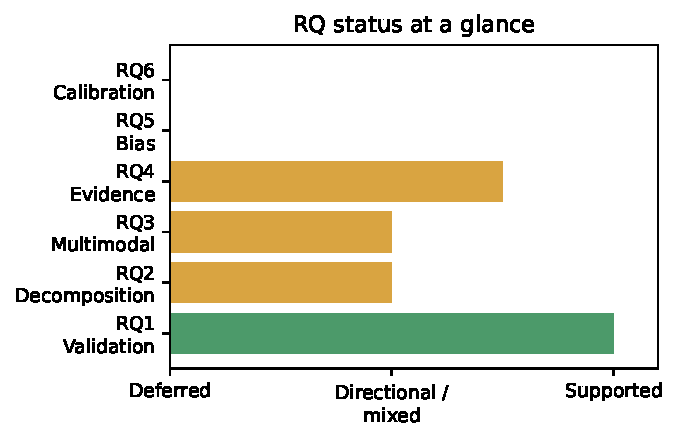
\includegraphics[width=0.95\linewidth]{figures/fig8_rq_status.pdf}
\caption{Status of each research question at a glance (green = supported,
amber = directional/mixed, red = deferred). Derived from
Table~\ref{tab:rqs}; not new data.}
\label{fig:rqstatus}
\end{figure}

This paper makes the following contributions, limited to what the
experiments in Sections~\ref{sec:results}--\ref{sec:bce} actually support:

\begin{enumerate}
\item \textbf{A held-out, Tier-1 evaluation benchmark and controlled
  baseline/counterfactual comparison} (Sections~\ref{sec:expmethodology}--
  \ref{sec:dataset}), the first evaluation against independent
  professional ground truth rather than development-time telemetry,
  holding model, search infrastructure, and (Section~\ref{sec:baselinefix})
  claim-extraction input constant so measured differences are
  attributable to downstream architecture, not to which configuration had
  an easier claim to reason about.
\item \textbf{A documented, fixed methodological confound in our own
  baseline design, reported with the same prominence as any other
  finding.} Baselines 1--3 had, in every run across this project, been
  given a clean, human-written claim summary rather than TruthLens's own
  extracted claim (Section~\ref{sec:baselinefix}), contradicting our
  stated methodology and inflating baseline performance. We fixed it and
  re-ran the comparison rather than silently correcting the number,
  reversing this program's headline result in the process.
\item \textbf{An empirical demonstration that verdict-label accuracy and
  \emph{support validity} are separable, independently-moving properties}
  (Section~\ref{sec:evidencevalidation}). Two general,
  ground-truth-independent validator fixes improved recall
  (16.7\%$\to$40\%, $n=9$, 100\% precision throughout) while leaving
  reel-level accuracy unchanged (2/6 before and after) -- outputs became
  measurably more supported by their own cited evidence without becoming
  more ``accurate'' by the bucket-matching standard.
\item \textbf{A claim-decomposition counterfactual analysis} isolating
  the clearest component-level result in this program, where aggregation
  demonstrably outperformed a simpler alternative (50.0\% vs.\ 25.0\%,
  $n=4$, Section~\ref{sec:ablation}).
\item \textbf{A four-way evidence-quality analysis} separating source
  -tier classification, topical relevance, fetch success, and
  usable-evidence extraction (Section~\ref{sec:evidencevalidation}):
  retrieval finds real, on-topic primary sources at a meaningfully higher
  rate (68.75\%) than usable-evidence rate (18.75\%) would suggest -- the
  bottleneck is source specificity, not retrieval relevance.
\item \textbf{A cross-referenced taxonomy of real failure modes}
  (Section~\ref{sec:failuremodes}), each found by running the complete
  system against real content end-to-end and fixed with a deterministic
  check and a regression test built from the case that surfaced it.
\item \textbf{\textsc{TruthLens-202}}: a 202-item held-out benchmark of
  real short-form political posts (X, Instagram, Facebook), each anchored
  to an independent professional fact-check via a verbatim evidence quote
  under a review-gated protocol, with 206 documented same-media
  cross-post relationships (Section~\ref{sec:truthlens202}). Its full
  composition and limitations -- LLM-performed annotation under author
  direction, $\sim$88\% single-source ground truth, and three
  domain-driven skews --
  are reported in full. We also contribute the first end-to-end result
  on it (Section~\ref{sec:tl202eval}): a local-only, \$0 configuration
  run over all 193 validation items, reported as a floor -- 34.7\% of
  posts reach a verdict, 29.9\% bucketed accuracy on those, and claim
  extraction identified as the binding constraint (65.3\%
  no-checkable-claim rate at 0\% infrastructure failure).
\end{enumerate}

TruthLens does not claim to have invented retrieval-augmented LLM
fact-checking, claim decomposition, source-credibility tiering, or
multimodal misinformation detection -- each independently pre-dates this
work, as Section~\ref{sec:relatedwork} discusses. Its contribution is the
specific combination of these mechanisms gated by deterministic,
non-LLM verification, evaluated against independent ground truth including
where that combination does not yet outperform a simpler alternative.

\section{TruthLens Architecture}
\label{sec:architecture}

TruthLens is a FastAPI backend with a PostgreSQL/pgvector datastore, a
Next.js review dashboard, and an object store (S3-compatible) for media
and rendered output. Figure~\ref{fig:architecture} shows the 9-stage
pipeline; no stage begins before the previous one has persisted its
output. Stage 1 (ingestion) downloads or accepts a video or photo,
transcribes audio, OCRs on-screen text at a fixed interval, and selects a
thumbnail (Section~\ref{sec:multimodal} covers the photo-post path).
Stage 2 (claim extraction) has an LLM decompose the transcript/OCR/
caption into atomic claims classified \texttt{factual}/\texttt{opinion}/
\texttt{prediction}/\texttt{satire}/\texttt{rhetorical}, with only
specific \texttt{factual} claims marked \texttt{verifiable}. Stage 3
(research planning) proposes 2--5 targeted search queries per verifiable
claim, explicitly requesting at least one primary-source-targeted query.
Stage 4 (search and fetch) runs each query and extracts full page text,
not just the snippet. Stage 5 (evidence analysis) has an LLM judge
stance (\texttt{supports}/\texttt{contradicts}/\texttt{provides\_context}/
\texttt{irrelevant}) per fetched source, grounded only in that source's
own extracted text. Stage 6 (verdict proposal) gives an LLM the claim and
its full evidence matrix and asks for a label, confidence, and cited
evidence IDs. Stage 7 is deterministic validation
(Section~\ref{sec:validation}). Stage 8 derives one reel-level verdict
from a fixed rule table over already-validated per-claim verdicts, not a
further LLM call. Stage 9 assembles a carousel from already-validated
database rows, with only headline phrasing and a short ``why'' paragraph
passing through one additional narrow, grounded LLM call each
(Section~\ref{sec:cascade}).

\begin{figure}[!t]
\centering
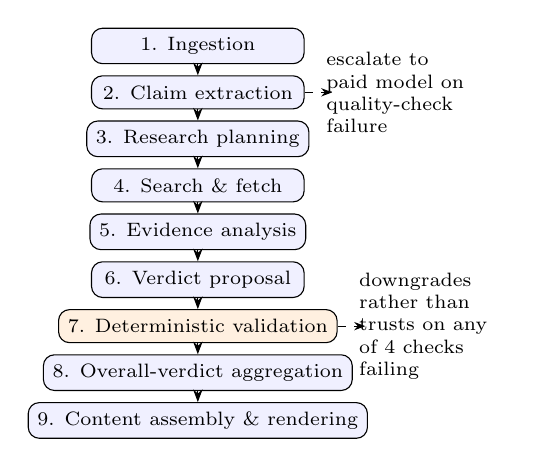
\begin{tikzpicture}[
  font=\scriptsize,
  stage/.style={draw, rounded corners, minimum width=2.7cm, minimum height=0.42cm, align=center, fill=blue!6},
  gate/.style={draw, rounded corners, minimum width=2.7cm, minimum height=0.42cm, align=center, fill=orange!12},
  arr/.style={-{Stealth[length=1.6mm]}}
]
\node[stage] (n1) {1. Ingestion};
\node[stage, below=0.14cm of n1] (n2) {2. Claim extraction};
\node[stage, below=0.14cm of n2] (n3) {3. Research planning};
\node[stage, below=0.14cm of n3] (n4) {4. Search \& fetch};
\node[stage, below=0.14cm of n4] (n5) {5. Evidence analysis};
\node[stage, below=0.14cm of n5] (n6) {6. Verdict proposal};
\node[gate, below=0.14cm of n6] (n7) {7. Deterministic validation};
\node[stage, below=0.14cm of n7] (n8) {8. Overall-verdict aggregation};
\node[stage, below=0.14cm of n8] (n9) {9. Content assembly \& rendering};
\draw[arr] (n1) -- (n2);
\draw[arr] (n2) -- (n3);
\draw[arr] (n3) -- (n4);
\draw[arr] (n4) -- (n5);
\draw[arr] (n5) -- (n6);
\draw[arr] (n6) -- (n7);
\draw[arr] (n7) -- (n8);
\draw[arr] (n8) -- (n9);
\node[align=left, right=0.15cm of n2, text width=1.9cm] {\scriptsize escalate to paid model on quality-check failure};
\draw[-{Stealth[length=1.4mm]}, dashed] (n2.east) -- ++(0.35,0);
\node[align=left, right=0.15cm of n7, text width=1.9cm] {\scriptsize downgrades rather than trusts on any of 4 checks failing};
\draw[-{Stealth[length=1.4mm]}, dashed] (n7.east) -- ++(0.35,0);
\end{tikzpicture}
\caption{The 9-stage TruthLens pipeline (Section~\ref{sec:architecture}).
No stage begins before the one before it has persisted its output. Stage 7
(orange) is the deterministic, non-LLM validation gate (Section
\ref{sec:validation}); five stages (2, 5, 6, and the two content
-generation calls inside stage 9, plus stage 5's newer sibling check) run
their own substantiveness check before accepting local-model output
(Section~\ref{sec:cascade}).}
\label{fig:architecture}
\end{figure}

\subsection{Source tiering}
Every retrieved source is scored along an 8-dimension weighted reliability
rubric and assigned to one of eight tiers: \texttt{primary\_government},
\texttt{primary\_legal}, \texttt{primary\_data}, \texttt{news\_wire},
\texttt{established\_news}, \texttt{academic}, \texttt{factcheck\_org}, or
\texttt{other}. Tier membership determines both which sources are eligible
to be surfaced as a claim's ``primary source'' citation on the rendered
carousel and, in aggregate, the reliability-weighted confidence of the
evidence matrix handed to the verdict-proposal stage. RQ4
(Section~\ref{sec:evidencevalidation}) evaluates this mechanism directly.
The eight dimensions' weights are hand-set manual priors, not derived
from any formal method or learned fit -- verified via git history to be
unmodified since before any evaluation dataset existed. A sensitivity
analysis against an unweighted or alternative rubric is unperformed,
named in Section~\ref{sec:futurework}.

\subsection{Multi-claim, reel-level verdicts}
TruthLens builds one fact-check per \emph{reel}, covering every verifiable
claim extracted from it -- collapsing several claims of differing
veracity into one verdict discards exactly the ``partially true,
partially misleading'' structure a reader needs. A fixed rule table
combines per-claim verdicts into the published carousel's one verdict
(Section~\ref{sec:aggregation}); Section~\ref{sec:ablation} tests whether
this multi-claim structure improves accuracy over the single
highest-importance claim alone.

\subsection{Multi-modal ingestion: video and photo posts}
\label{sec:multimodal}
When the video downloader reports no video stream, the pipeline falls
back to the post's Open Graph metadata (image URL, caption, engagement
counts) fetched directly from the page. A \texttt{media\_type} field
drives branching at exactly one point: audio/transcription are skipped
for a photo, but OCR and vision-context needed no new code, since both
already operate on a plain list of image paths -- a photo is a
one-element case of the same interface video frames already satisfy.
Section~\ref{sec:multimodalanalysis} evaluates claim coverage across this
system's three real input-modality conditions.

\subsection{Making the model's output more supportable}
\label{sec:methodology}
We make precise, in place of the vaguer word ``trustworthy,'' a single
construct used throughout this paper: a verdict has \textbf{support
validity} to the extent that every specific, checkable assertion in it --
cited evidence IDs, the sources they point to, reasoning numbers, and the
logical relationship between reasoning and label -- can be verified
against data already in the pipeline's evidence matrix, without a second
model judgment. Support validity is deliberately narrower than, and does
not imply, label accuracy or general absence of hallucination: a verdict
can have perfect support validity and still be wrong, if the model
correctly cited evidence it misinterpreted, or if retrieval never found
the right evidence at all (Section~\ref{sec:evidencevalidation}'s
four-way metric addresses that). Sections~\ref{sec:results}--\ref{sec:bce}
evaluate whether the mechanisms below actually make this checkable.

\subsubsection{Deterministic evidence-grounding validation}
\label{sec:validation}
After the verdict-proposal LLM call returns a structured
\texttt{VerdictProposal} (label, confidence, reasoning, cited evidence
IDs), TruthLens runs four checks against data already in the database, none
of which invoke an LLM:

\begin{itemize}
\item \textbf{Citation existence:} every ID in \texttt{cited\_evidence\_
  ids} must correspond to an evidence row that was actually passed to the
  model in its evidence matrix.
\item \textbf{Source-fetch existence:} every cited evidence row's source
  must have a stored, successfully fetched full-text passage -- a citation
  cannot point at a source the pipeline only planned to fetch.
\item \textbf{Number grounding:} every numeral appearing in the model's
  \texttt{reasoning\_summary} is extracted and checked for appearance in at
  least one cited source's stored passage text. UUID-shaped hex sequences
  (from internal citation markup) are stripped before number extraction --
  a real bug, described in Section~\ref{sec:failuremodes}, in which digits
  from a cited evidence ID's own UUID were being extracted as apparent
  ``unsupported statistics.''
\item \textbf{Reasoning/label consistency (new).} A verdict whose own
  \texttt{reasoning\_summary} states that no reliable evidence was found
  (matched against a fixed phrase list, e.g.\ ``does not provide any
  reliable,'' ``no reliable sources'') but whose label is a confident
  value other than \texttt{UNVERIFIED} is downgraded to
  \texttt{UNVERIFIED}. Added in direct response to Section
  \ref{sec:evidencevalidation}'s finding that this specific pattern was
  the largest single category of validator false negative; its
  circularity as a threat to validity is disclosed, not hidden, in
  Section~\ref{sec:evidencevalidation}.
\end{itemize}

These four checks are the entire current operationalization of support
validity -- deliberately not a proxy for evidence-to-claim topical
relevance (Section~\ref{sec:evidencevalidation}'s job), evidence-to
-reasoning stance correctness (human-audited only, a named gap), or
entity consistency (not yet implemented, Section~\ref{sec:futurework}). A
verdict that fails any check is \emph{downgraded}, not discarded:
persisted with a non-\texttt{passed} \texttt{validation\_status}, an
appended \texttt{[VALIDATION NOTE: ...]}, and excluded from citation
lists.

\texttt{UNVERIFIED} means the system genuinely searched and found
insufficient evidence; a distinct \texttt{RESEARCH\_FAILED} status is
raised only when \emph{all} queries fail at the infrastructure level, and
a publication gate refuses to build a fact-check from it -- distinguishing
``I don't know'' from ``I could not check.''

\subsubsection{Verification-gated model cascading}
\label{sec:cascade}
Every stage defaults to a free, local model. Five stages run a
deterministic \emph{substantiveness check} before accepting local-model
output -- e.g.\ vision-context requires its \texttt{scene\_description}
to clear a 0.20 word-overlap-with-prompt threshold (calibrated against
every real garbled/coherent example collected: garbled 0.26--0.29,
coherent 0.00--0.12), and evidence analysis requires a non-empty
per-source \texttt{explanation} (added after Section
\ref{sec:evidencevalidation} found 47.1\% empty). On failure, the call
retries once against a paid model (Gemini) with an identical prompt --
unlike a classic cascade \cite{chen2023frugalgpt}, the trigger is a
deterministic per-stage predicate, not a learned confidence estimate.
Full per-stage thresholds and illustrative firing-rate telemetry:
Appendix~\ref{sec:appendixarchitecture}.

\subsubsection{Deterministic aggregation and grounded corrections}
\label{sec:aggregation}
Once every claim has a verdict, TruthLens derives one reel-level verdict
via a fixed rule table over the \emph{set} of per-claim labels (weighted
by importance $\geq 0.5$ as ``major''): a plain combinatorial function,
not a further LLM call, keeping the published carousel's headline verdict
auditable from already-validated per-claim verdicts
(Section~\ref{sec:ablation} evaluates this mechanism directly). Optional
\texttt{corrected\_fact}/\texttt{context\_note} fields, held to the same
evidence-grounding rule, are also produced and invalidated alongside the
parent verdict on any validation failure; full rule table and field
details: Appendix~\ref{sec:appendixarchitecture}.

\subsection{Stage 10: human-approval-gated publishing}
\label{sec:publishing}
Stage 9's rendered carousel is not posted automatically. A tenth stage,
outside the 9-stage accuracy pipeline Figure~\ref{fig:architecture}
diagrams and outside every research question this paper evaluates,
publishes an \texttt{approved} fact-check to a real Instagram account via
the official Meta Graph API's Content Publishing endpoints -- no browser
automation or unofficial API of any kind, matching this project's stated
Terms-of-Service-compliance posture (\texttt{docs/API\_REQUIREMENTS.md}~\S7). The state machine
(\texttt{researching}$\to$\texttt{ready\_for\_review}$\to$\texttt{approved}
$\to$\texttt{published}) enforces a human decision at
\texttt{ready\_for\_review}: nothing reaches Instagram without an explicit
reviewer approval, and approval and publish are two separate API calls
against two separate database rows (a \texttt{GeneratedPost} created at
approval time, a \texttt{PublishingJob} created at publish time) rather
than one combined action, specifically so a failed Graph API call cannot
silently re-trigger a duplicate approval or a double post. The publish
call itself is a fixed six-step sequence per Instagram's own documented
protocol: create one media container per slide, poll each until
Instagram's servers report \texttt{FINISHED}, create a carousel container
referencing all four, poll it, then publish and retrieve the permalink --
each step individually retried (three attempts, exponential backoff) but
the overall sequence not idempotent, which is what the approval/publish
split above is defending against. Cost is \$0 (Meta's standard platform
terms; the observed constraint is a rate limit, not a price -- roughly 25
\texttt{media\_publish} calls per 24 hours per account, against which this
project's own configured cap of 12 posts/day leaves real but not
lavish margin).

This stage has existed since the project's initial build but, unlike
every accuracy-pipeline stage above, had zero test coverage before this
pass -- a real gap for the one piece of code with an external, real-world,
hard-to-fully-undo side effect. 18 tests were added: the full six-step
Graph API sequence against a mocked HTTP boundary (container creation,
ready-polling including a timeout case, carousel creation, publish,
permalink retrieval), both real error shapes the Graph API actually
returns (an HTTP error status, and a \texttt{200} response carrying an
\texttt{error} object), the 2--10 item carousel-size guard, and --
against a real row graph, not mocks, for everything except the Graph API
call itself -- the already-published refusal, the missing-access-token
refusal, and that a Graph API failure marks the publishing job
\texttt{failed} with a real stored error rather than leaving it stuck or
incorrectly marking the fact-check published anyway. No test exercises a
live Instagram account: doing so requires the operator to complete a
one-time account-linking step (an Instagram Business account linked to a
Facebook Page, added as a Tester on a Meta developer app -- free, but
outside this codebase, documented in
\texttt{docs/API\_REQUIREMENTS.md}~\S1) that had not been completed as of
this writing (Section~\ref{sec:conclusion}).

\section{Experimental Methodology}
\label{sec:expmethodology}

\subsection{Central research question and design}
The central question motivating this evaluation: can a verification-gated,
evidence-grounded architecture reduce unsupported fact-checking outputs
while preserving or improving factual correctness in short-form political
media? We answer this via a controlled comparison across five system
configurations, all run against the same underlying local model
(\texttt{llama3.2} via Ollama) and, where the configuration has search
access at all, the same search provider (DuckDuckGo) TruthLens itself uses
in production -- holding model and search-infrastructure quality constant so
that a measured difference is attributable to architecture, not to a
cheap-model-vs.-expensive-model confound.

\subsection{System configurations}
Five configurations, all on \texttt{llama3.2}: \textbf{B1 (LLM-only)} --
claim $\to$ verdict, no search/evidence/validation. \textbf{B2
(Search+LLM)} -- claim $\to$ one DuckDuckGo search (top-5 snippets, no
full-page fetch) $\to$ verdict; the claim is passed to search verbatim,
no research-planning stage, the single most important difference from B3
and TruthLens. \textbf{B3 (Search+RAG+LLM)} -- adds full-page fetch/
extraction over the same results, isolating retrieval depth from
decomposition and per-source analysis. \textbf{B4 (TruthLens minus
validation)} -- the real pipeline with \texttt{validate\_verdict()}'s
outcome recorded but never applied (a runtime flag, \texttt{SKIP\_VALIDATION},
not a forked codepath), the primary RQ1 ablation. \textbf{Full TruthLens}
-- unmodified, at the frozen evaluation tag. Decomposition, source
tiering, per-source analysis, and validation exist only in the full
system; Baselines 1--3 operate on TruthLens's own already-extracted
claim, since claim extraction itself is RQ3's job, not RQ2's. A real
infrastructure bug was found and fixed while building B2/B3 (the first
draft silently inherited TruthLens's own Gemini-fallback mechanism via a
shared provider factory, caught during smoke testing;
Section~\ref{sec:failuremodes}).

\subsection{Ablations, metrics, and held-out discipline}
Beyond B4 (RQ1), two further ablations: a \textbf{source-tier ablation}
(domain-restricted vs.\ unrestricted retrieval,
Section~\ref{sec:evidencevalidation}) and a \textbf{claim-decomposition
ablation} (Section~\ref{sec:ablation}), computed from already-collected
verdict data at zero additional LLM cost. Every proportion is reported
with its exact numerator/denominator and a 95\% Wilson CI; paired
comparisons use McNemar's exact test with the raw contingency table, never
a bare $p$-value; accuracy uses a fixed \texttt{VerdictLabel}-to-ground
-truth bucketing where \texttt{UNVERIFIED} never counts as a match. Full
formulas are fixed in advance in \texttt{METRICS.md} and not altered
after seeing results. The dataset (Section~\ref{sec:dataset}) is checked
item-by-item against already-ingested development content and excluded
on any match; no prompt, threshold, or model choice was changed based on
dataset contents or performance after an item was added -- the two
general fixes in Section~\ref{sec:evidencevalidation} are deliberately
\emph{ground-truth-independent}, with that distinction's limits argued
explicitly, not asserted. Two tagged freezes (dataset before Baselines
1--3; system code before the held-out run) mean any later code change is
logged, never silently applied.

\subsection{Honest scope reductions}
\label{sec:honestscope}
Stated rather than hidden: \textbf{9 items, not 50--100} (a pilot found
$\sim$8\% hit rate for a usable Tier-1 candidate; 20--30 items would need
250--375 more articles checked, Section~\ref{sec:dataset}).
\textbf{Single annotator, no IAA statistic} -- Tier-1 ground truth is a
professional organization's own verdict, authored by no one on this
project; any Tier-2 judgment used (draft claim-coverage/evidence
-relevance labels only, never a headline verdict) is explicitly marked as
such. \textbf{RQ3, RQ5, RQ6 reported as directional or deferred}, not
generalizable rates. \textbf{No $p$-values from tests assuming a sample
size this program does not reach} -- Wilson intervals and McNemar's exact
test only, reported as uncertainty descriptions, not significance claims.

\section{Dataset and Annotation}
\label{sec:dataset}

This work uses two disjoint held-out sets. The \textbf{9-item comparison
set} (Sections~\ref{sec:dataset}.B--F) is the frozen \texttt{dev} split
against which every controlled result in Section~\ref{sec:results} and the
foundation-phase experiments (Section~\ref{sec:foundationphase}) are
computed; it is small by deliberate, disclosed choice
(Section~\ref{sec:honestscope}) and is never re-touched.
\textbf{\textsc{TruthLens-202}} (Section~\ref{sec:truthlens202}) is a
separate, larger \texttt{validation} split, built after the frozen
comparison, that the platform-scope and sourcing findings of this program
made feasible. It is evaluated end-to-end once here, in a single
local-only configuration (Section~\ref{sec:tl202eval}); that number is
reported as a floor and is kept strictly separate from the frozen
\texttt{dev}-split results, which it does not affect.

\subsection{Ground-truth tiers}
\textbf{Tier 1 (used for every item in this evaluation):} the claim in the
Instagram post has already been verdicted by an independent professional
fact-checking organization, and that organization's article demonstrably
references or embeds this specific post, not merely a similar claim
elsewhere. Ground truth is their published verdict, with the article URL
stored for auditability. \textbf{Tier 2 (specified, not used for any
headline verdict in this evaluation):} no professional fact-check exists;
a project annotator labels directly from primary sources under a documented
protocol. No item is ever labeled by TruthLens itself, or by any LLM, and
then used as ground truth.

\subsection{The 9-item benchmark}
Table~\ref{tab:dataset} lists every item. All 9 are Tier 1, sourced from
BOOM Live, Alt News, and Factly. item-0003 (a CJP-investigated,
AI-generated visual claim) could not be ingested after three independent
attempts across this program (a persistent Instagram-side ``empty media
response''), and is excluded from every table in this paper, not scored as
a failure.

\begin{table*}[!t]
\caption{Held-out benchmark: 9 Tier-1 items (all sourced independently of TruthLens or its developer)}
\label{tab:dataset}
\centering
\footnotesize
\begin{tabular}{lllll}
\toprule
ID & Ground truth & Source & Political actor & Claim type \\
\midrule
item-0001 & FALSE & BOOM Live & BJP & provenance \\
item-0002 & FALSE & Alt News & Karni Sena & provenance (visual) \\
item-0003$^\dagger$ & FALSE & BOOM Live & CJP & visual (AI-generated) \\
item-0004 & TRUE & BOOM Live & Delhi Police (government) & provenance \\
item-0005 & MISLEADING & Factly & Congress & provenance \\
item-0006 & FALSE & BOOM Live & none (disaster misinfo) & event (visual) \\
item-0007 & FALSE & Alt News & BJP & misleading context \\
item-0008 & FALSE & Alt News & AAP & quote \\
item-0009 & FALSE & Alt News & BJP & provenance \\
\bottomrule
\end{tabular}
\\[2pt]
\raggedright\footnotesize $^\dagger$Never successfully ingested; excluded from all analyses.
\end{table*}

\subsection{Sourcing method and hit rate}
Items were sourced by searching professional fact-checking outlets for
articles that embed a still-live Instagram post, prioritizing coverage
gaps in claim type, language, and political actor across three sourcing
passes. The method's real, load-bearing constraint is a $\sim$8\% hit
rate (2 of the first 26 fact-check articles checked yielded a usable,
still-live, directly-embedded post) -- most professional fact-checks
either do not embed the specific post, or it has since been taken down.
Every accepted item's content hash is checked against already-ingested
development data and excluded on any match.

\subsection{Inter-annotator agreement}
No IAA statistic is computed, and none is fabricated to fill this gap.
Tier-1 ground truth does not have an ``annotator'' in the IAA sense -- the
label is a single organization's single published verdict, and
introducing a second in-project annotator to re-judge it would defeat the
purpose of using independent ground truth. No Tier-2 items exist in the
frozen dataset, so the condition under which IAA would be meaningful does
not currently arise; if Tier-2 items are added with only one available
annotator, this will continue to be reported as ``single-annotator ground
truth, no IAA computed,'' not papered over with an unearned kappa
statistic.

\subsection{Composition gaps, disclosed}
\label{sec:datasetgaps}
Five of 9 items are \texttt{provenance}-type claims; \texttt{statistic},
\texttt{law\_policy}, \texttt{historical}, and \texttt{true\_claim} remain
unrepresented after three sourcing passes -- plausibly, though unprovenly,
a property of which claim types concentrate on Instagram versus other
platforms in this domain. Seven of 9 items are \texttt{FALSE}, likely
reflecting that fact-checkers publish far more debunks than confirmations;
only item-0004 is \texttt{TRUE}. Two items (item-0007, item-0008) have
confirmed Hindi/mixed spoken content, still a thin representation of the
project's stated multilingual target. BJP has 3 items (the most of any
actor, alongside 6 single-item actors), but none form a controlled
topic/structure/difficulty match against another actor, which is why RQ5
(Section~\ref{sec:bce}) is deferred rather than attempted at
$n=1$-per-comparison.

\subsection{\textsc{TruthLens-202}: a larger held-out benchmark}
\label{sec:truthlens202}

The 9-item comparison set above is frozen and never expanded. Separately,
this program built a larger held-out corpus, \textsc{TruthLens-202}, for
end-to-end evaluation. It comprises 202 real short-form political
posts: the 9 comparison items form its \texttt{dev} split, and 193 newly
collected items form a \texttt{validation} split, evaluated once in this
paper (local-only configuration, Section~\ref{sec:tl202eval}) and kept
separate from the frozen \texttt{dev}-split results. We describe how it
was built, its composition, and its limitations in full, because the way
an evaluation set is constructed is itself a claim that should be
checkable.

\subsubsection{Why the platform scope was relaxed}
The five earlier sourcing passes (Sections~\ref{sec:dataset},
\ref{sec:foundationphase}, \ref{sec:massSourcing}) restricted candidates
to Instagram. Section~\ref{sec:massSourcing} measured the cost of that
restriction directly: across roughly 3{,}600 candidates screened over
five Indian fact-checker archives, the blended yield of a usable
Instagram-native misinformation-source post was on the order of one per
900, an order of magnitude below the original manual-sourcing estimate.
That finding, first observed qualitatively in
Section~\ref{sec:multimodalanalysis} (most of this pattern's false claims
are attached on X/Twitter, not Instagram) and then confirmed
quantitatively at volume, is what motivated relaxing the constraint: not
a preference for scale over rigor, but a measured structural property of
where this misinformation actually recirculates. \textsc{TruthLens-202}'s
\texttt{validation} split therefore admits posts from any platform whose
media is retrievable through an official/sanctioned path (X/Twitter,
Facebook, Instagram, and in principle YouTube and TikTok), while holding
every other bar constant: a real professional fact-check must establish
the claim and verdict, the post must still be live and retrievable, and
the post's own text must itself assert the false claim rather than merely
being cited as evidence or the true original.

\subsubsection{Sourcing pipeline}
An automated pipeline crawls the same fact-checker archives plus, newly,
Lead Stories, Full Fact and Check Your Fact; extracts every embedded
social-media URL (widget-permalink and plain-link forms across all five
platforms); verifies retrievability with \texttt{yt-dlp} and pulls the
post's own caption and uploader directly from platform metadata, never
inferred from the article; deterministically skips the fact-checker's own
account and a fixed list of official government/platform fact-check
handles; and passes each survivor to a local \texttt{llama3.2}
structured call that decides, given the fact-check article text and the
post's real caption, whether the post's own text asserts the debunked
claim. 11{,}544 candidates across seven archives were screened this way.
The judge is a screening filter only: its output is never ground truth.

\subsubsection{Review-gated annotation protocol}
Every candidate the screen accepts is then adjudicated by a single
reviewer who reads the professional fact-check article in full and
records four fields: (i)~a standalone one-sentence statement of the
debunked claim, in English; (ii)~a verdict mapped to the paper's
label taxonomy; (iii)~a verbatim quote or close paraphrase from the
article that establishes that verdict -- the ground truth is anchored to
this quote, not to the reviewer's or the screen's judgment; and
(iv)~claim type, language, and political actor. A candidate is
\emph{deferred} rather than promoted when it is a cross-post of an
already-promoted item (kept as a documented relationship, not discarded),
when the specific post's own text cannot be retrieved to confirm what it
asserts, or when the fact-check article is a report on real incidents
rather than a debunk. A candidate is \emph{rejected} when the screening
judge misfired on an official, news-agency, or rebuttal account. The
reviewer's decision log holds 372 adjudicated candidates: 166 marked
\emph{promote} (of which 165 completed end-to-end ingestion into the
\texttt{validation} split), 148 \emph{deferred}, and 58 \emph{rejected}.
Counting earlier passes as well, 206 candidates carry a
\texttt{deferred\_crosspost} marker recording that they duplicate a
promoted item's underlying media under a different account. Twenty-eight
further \texttt{validation} items predate this protocol (a pre-protocol
automated batch): 9 are flagged
\texttt{annotation\_status=needs\_review} and 19 carry no review status,
all pending the same adjudication. This gives $165+28=193$
\texttt{validation} items.

\subsubsection{Composition}
Table~\ref{tab:tl202} gives the full distribution of all 202 items.
Three skews are structural to this domain, not sourcing artifacts, and
any evaluation on this set must account for them:
\textbf{(1)~label}: 83\% \texttt{FALSE}, because professional
fact-checkers publish far more debunks than confirmations -- balanced
accuracy or per-class $F_1$, not raw accuracy, is the appropriate
end-to-end metric (an always-\texttt{FALSE} predictor scores 83\%);
\textbf{(2)~platform}: 80\% of items are from X/Twitter, the measured
locus of this pattern and also where \texttt{yt-dlp} retrieval succeeds
most reliably without authentication; \textbf{(3)~claim type}: 80\% are
\texttt{provenance}-type (authentic footage recirculated with a false
date, place, or context), the dominant 2024--2025 Indian pattern.
A fourth, non-structural concentration is disclosed as a limitation
below: $\sim$88\% of the \texttt{validation} split's ground truth comes
from a single organization, Alt News.

\begin{table}[!t]
\caption{\textsc{TruthLens-202} composition (202 items: 9 \texttt{dev} + 193 \texttt{validation})}
\label{tab:tl202}
\centering
\footnotesize
\setlength{\tabcolsep}{3pt}
\begin{tabular}{@{}p{0.20\linewidth}p{0.74\linewidth}@{}}
\toprule
Dimension & Distribution \\
\midrule
GT label & \texttt{FALSE} 167 (82.7\%), \texttt{MISLEADING} 30, \texttt{TRUE} 5 \\
Platform & X/Twitter 161 (79.7\%), Instagram 25, Facebook 16 \\
Language & English 146, Hindi 52, Bengali 3, Arabic 1 \\
Claim type & \texttt{provenance} 161 (79.7\%), \texttt{event} 12, \texttt{misleading\_context} 12, \texttt{quote} 11, other 6 \\
Media & video 200, photo 2 \\
Fact-checker (val.) & Alt News 170, Lead Stories 14, BOOM 4, Check Your Fact 2, others 3 \\
Modality (val.) & caption 192/193, audio 163/193, OCR 91/193; visual-context analysis deferred on 115 \\
Cross-post links & 206 documented same-media relationships \\
\bottomrule
\end{tabular}
\end{table}

\subsubsection{Leakage and split discipline}
The 9 \texttt{dev} items and the 193 \texttt{validation} items are
disjoint by construction and by content hash. Within the corpus, an
automated check flags any \texttt{factcheck\_url} or
\texttt{media\_content\_hash} that appears in more than one split (none
do), and the 206 cross-post markers make same-underlying-media
relationships explicit rather than leaving near-duplicate posts to be
treated as independent examples. No prompt, threshold, or model choice
in this paper was tuned on \textsc{TruthLens-202}; it did not exist when
the frozen comparison was run.

\subsubsection{Limitations, stated plainly}
\textbf{(1)~One configuration evaluated so far.} All 193
\texttt{validation} items have been run end-to-end, but only in the
local-only configuration (Section~\ref{sec:tl202eval}); the larger-local
-model, vision-first, and cloud-escalation configurations are not yet
measured against this split. \textbf{(2)~Two axes of ground-truth provenance, and a selection
circularity.} Ground truth here has two independent dimensions that must
not be collapsed. \emph{Verdict provenance} is uniform: every one of the
202 items' \texttt{TRUE}/\texttt{FALSE}/\texttt{MISLEADING} verdict is an
independent professional fact-checking organisation's published finding,
anchored to a recorded verbatim quotation from its article.
\emph{Annotation provenance} is not. The 9 \texttt{dev} items were
labelled directly from the fact-checker's own published ClaimReview
(\texttt{annotation\_provenance = professional-factcheck-direct}). For
the 193 \texttt{validation} items, by contrast, the claim phrasing, the
mapping of the fact-checker's verdict onto this paper's label taxonomy,
and the promote/defer/reject decision were \textbf{performed by a large
language model under the author's direction and applied in batch} --
not drafted by a model and then adjudicated item-by-item by a human.
165 items carry that provenance
(\texttt{llm-assisted-review}); the remaining 28 predate the protocol
(\texttt{pre-protocol-automated}) and are weaker still. We state this
plainly rather than describing the process as human annotation with
model assistance, which would overstate the human role. No
inter-annotator agreement statistic is available and none is fabricated.

A sharper form of the same concern is \textbf{selection}. The screening
model that decided which of 11{,}544 candidates entered the corpus was
\texttt{llama3.2} -- the same model subsequently evaluated on it
(Section~\ref{sec:tl202eval}). The evaluee therefore participated in
choosing its own test set. The screen accepted a candidate when the
post's own text asserted the debunked claim, so the bias runs
\emph{toward} items this model can parse; a random sample of real posts
should, if anything, be harder. That direction matters for how the
result is read: the reported 29.9\% bucketed and 22.2\% balanced
accuracy are best understood as a \textbf{favourably-selected floor},
not a pessimistic outlier. It does not make the corpus unusable -- the
verdicts remain independently sourced -- but no number on this split
should be treated as a validated headline until a second independent
annotator and a screen drawn from a different model family are in place
(Section~\ref{sec:futurework}). \textbf{(3)~Source concentration.}
$\sim$88\% of \texttt{validation} ground truth is Alt News's, because the
other archives yielded far less under the same bar (Lead Stories: $\sim$77\%
of its candidates had media already taken down; regional-language
archives produced almost nothing against an English-centric screening
judge; Full Fact and Check Your Fact mostly fact-check politician
statements rather than recirculated posts). \textbf{(4)~Deferred
visual analysis.} 115 \texttt{validation} items were ingested without the
vision-context stage (a $\sim$10-minute-per-item local model call that
produced low-value output on compressed social-video keyframes);
\texttt{visual\_information\_available} is recorded as null, not guessed,
for those, pending a backfill pass. \textbf{(5)~Domain and language.}
Still Indian political short-form content, now with a Hindi share
(26\%) closer to the stated multilingual target but still English-majority.
Full construction detail, and every promoted/deferred/rejected
candidate's recorded reasoning:
\texttt{research/dataset/TruthLens\_Dataset.xlsx} and the
\texttt{candidates\_v3\_*.jsonl} provenance files.

\section{Results}
\label{sec:results}

\subsection{A methodological correction, reported before the headline
number itself}
\label{sec:baselinefix}
A skeptical post-submission audit of this program's own experimental
design (full trail: \texttt{research/AUDIT\_REPORT.md}) found that
Baselines 1--3, in every run across this entire project, had been given
\texttt{items.jsonl}'s hand-written claim summary -- prose written during
dataset construction by a human who had already read the professional
fact-check -- rather than the claim actually extracted by TruthLens's own
claim-extraction stage, contradicting this paper's own stated methodology
(Section~\ref{sec:expmethodology}). The bug traced to a single,
never-modified helper function written on the first day baselines were
built. Because TruthLens's own extraction is often noisy or, on two of
six items, empty, this gave baselines a systematically cleaner input than
TruthLens itself ever worked with, for the entire program, undetected
until this audit.

We fixed it rather than merely disclosing it: Baselines 1--3 were re-run
against TruthLens's own real extracted claims (available for the same 6
items the paired comparison already uses -- item-0003 has no extraction
at all; items 0008/0009 remain excluded as before), one baseline call per
real extracted claim, aggregated with the identical deterministic rule
(\texttt{derive\_overall\_verdict()}) TruthLens itself uses. This holds
claim extraction constant across every configuration for the first time
in this program. Full item-by-item reconstruction:
\texttt{research/RECONSTRUCTED\_RESULTS.md}. \textbf{We report this
correction with the same prominence as the result it changes: a
methodology bug that inflated a baseline's apparent performance relative
to our own system is exactly the kind of finding Rule~1 of our own
governing protocol exists to surface, not bury.}

\subsection{Headline finding, corrected}
\textbf{On the paired six-item comparison, once claim input is held
constant, full TruthLens (33.3\%, 2/6) beats Baseline 1 (0.0\%, 0/6) and
Baseline 3 (0.0\%, 0/6) outright, and trails only Baseline 2
(50.0\%, 3/6) -- by 16.7 points, not the 33.4-point gap the uncorrected
comparison showed.} This reverses this program's previous headline
finding (Baseline 2 66.7\%, Baseline 3 50.0\%, both ahead of TruthLens).

\begin{table}[!t]
\caption{Paired comparison, identical 6 items, before and after the claim-input fix}
\label{tab:table2}
\centering
\scriptsize
\setlength{\tabcolsep}{4pt}
\begin{tabular}{lrrl}
\toprule
Config & Superseded & Corrected & 95\% CI \\
\midrule
B1: LLM-only & 0.0\% & 0.0\% & [0.0, 39.0] \\
B2: Search+LLM & 66.7\% & 50.0\% & [18.8, 81.2] \\
B3: Search+RAG+LLM & 50.0\% & 0.0\% & [0.0, 39.0] \\
Full TruthLens & 33.3\% & 33.3\% & [9.7, 70.0] \\
\bottomrule
\end{tabular}
\end{table}

\begin{figure}[!t]
\centering
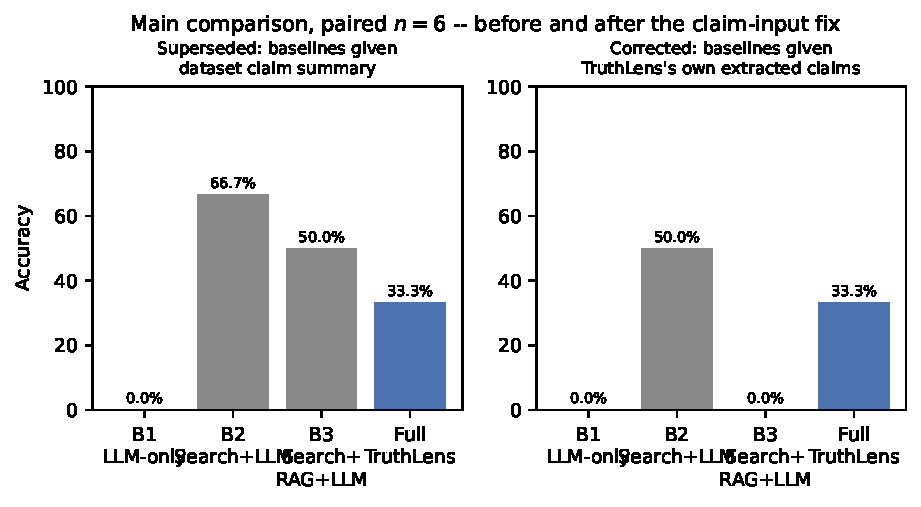
\includegraphics[width=\linewidth]{figures/fig2_main_results.pdf}
\caption{Table~\ref{tab:table2} plotted, superseded vs.\ corrected.
The reversal is concentrated in items where baselines had been implicitly
handed a claim to reason about that TruthLens itself never produced.}
\label{fig:mainresults}
\end{figure}

Item-by-item, the corrected picture:
\begin{itemize}
\item \textbf{item-0006, item-0007:} full TruthLens outputs
  \texttt{UNVERIFIED} on both because claim extraction found \emph{zero
  verifiable claims} for either (Section~\ref{sec:multimodalanalysis}:
  item-0006's transcript is garbled nonsense; item-0007's is degraded and
  repetitive). Under the superseded method, Baseline 2 had been handed a
  clean claim summary anyway and happened to guess \texttt{MOSTLY\_FALSE},
  matching ground truth. Corrected, every baseline receives the same
  nothing TruthLens received and also outputs \texttt{UNVERIFIED} -- a
  shared reflection of a real coverage gap, no longer a baseline-only
  advantage.
\item \textbf{item-0004:} Baseline 2 uniquely gets this right
  (\texttt{MOSTLY\_TRUE}); TruthLens's wrong verdict is the exact
  validator false negative Section~\ref{sec:evidencevalidation} already
  identifies. Baselines 1 and 3 also get this wrong.
\item \textbf{item-0005:} every configuration gets this wrong -- ground
  truth is \texttt{MISLEADING}, a bucket nothing landed in.
\item \textbf{item-0001, item-0002:} TruthLens and Baseline 2 agree (both
  correct). Baselines 1 and 3 get \emph{both} wrong under the corrected
  method, having gotten both right under the superseded one -- their
  earlier apparent success was partly an artifact of cleaner claim input,
  not evidence their reasoning handles TruthLens's own messier extracted
  claims equally well. Baseline 3 (full-page-text RAG) in particular
  moves from correct to incorrect on both, a directional signal
  (unverified at this $n$) that concatenating full page text may compound
  confusion for a small local model rather than compensate for it.
\end{itemize}

\textbf{McNemar analysis} (paired, $n=6$, Baseline 2 vs.\ Full TruthLens,
corrected): both-correct $=2$ (item-0001, item-0002), both-wrong $=3$
(item-0005, item-0006, item-0007), Baseline-2-only-correct $=1$
(item-0004), TruthLens-only-correct $=0$. One discordant pair; exact
McNemar $p=1.0$ -- still completely uninformative at this $n$, reported
for the same reason as before: completeness, not evidence. Against
Baselines 1 and 3, TruthLens now has zero discordant pairs favoring
either baseline (both are strictly dominated on this sample).

This is not a claim that TruthLens's architecture is unconditionally
better than a single-shot baseline; it is a claim that once the one
confound this audit found is removed, TruthLens is competitive with, and
mostly ahead of, the baselines it is compared against on this specific,
tiny, real sample -- and that the previous, opposite-looking result was
substantially an artifact of an experimental design bug, not a property
of the architecture. Section~\ref{sec:ablation} separately shows
decomposition helped once claim extraction produced multiple claims to
aggregate; the remaining deficit against Baseline 2 traces to
claim-extraction \emph{coverage} on hard audio (items 0006/0007) and one
validator false negative (item-0004), not a general disadvantage.

\textbf{The earlier, retired "each configuration's own full $n=9$ run"
table} (superseded by Table~\ref{tab:table2} above) is not cited as
evidence for any claim going forward and is retained only for the
historical record, in Appendix~\ref{sec:appendixsuperseded}.

\subsection{A real gap found and fixed during the six-item re-run, and known
disclosed gaps}
Extending the pipeline run to items 0008/0009 hit a genuine
\texttt{MissingGreenlet} crash -- the same bug class already fixed once in
production code -- after a per-claim exception handler called
\texttt{db.rollback()}, the next line's synchronous attribute access on an
already-expired ORM object crashed the whole script instead of recording
just that one claim's failure. Fixed by capturing needed values before the
try block, matching the earlier production fix's pattern; re-verified
live, the script then completed without crashing
(Section~\ref{sec:failuremodes}). Items 0008/0009's full-TruthLens
condition remains blocked by a real Gemini free-tier quota exhaustion,
confirmed live (two consecutive 429s, one from evidence-analysis
escalation, one from claim-extraction escalation) -- an external,
time-of-day resource constraint, not a system defect. Baselines 1--3
completed for both items (no Gemini dependency by design). Per-class F1
and full precision/recall breakdowns are not computed at this sample
size, where several label classes appear 0--1 times and per-class F1
would mostly be undefined or single-observation -- a scope decision, not
an omission dressed up with misleadingly precise zeros and ones.

\subsection{\textsc{TruthLens-202}: local-only end-to-end evaluation ($n=193$)}
\label{sec:tl202eval}
The frozen six-item comparison above measures the architecture against
its baselines under a controlled claim input. It says nothing about how
the deployed system behaves on a large, uncurated sample of the content
it targets. \textsc{TruthLens-202}'s \texttt{validation} split
(Section~\ref{sec:truthlens202}) is that sample, and this subsection
reports the first end-to-end run over all 193 of its items.

\paragraph{Configuration and what it measures}
The run uses the \emph{local-only} configuration: every LLM stage
(claim extraction, research planning, evidence analysis, verdict) on the
local \texttt{llama3.2} 3B model, keyless DuckDuckGo search, and
\emph{no} cloud escalation -- \texttt{GEMINI\_API\_KEY} unset, so every
quality-retry path in the code is inert. This is the \$0, no-API-key,
no-rate-limit configuration the project targets, and it is the honest
floor: any cloud escalation can only raise these numbers. Ingestion was
not re-run (each item keeps the real transcript/OCR from its promotion
pass); the run executes the exact production stage functions in the
\texttt{orchestrator.analyze\_reel} order, then the deterministic
\texttt{derive\_overall\_verdict}. Full per-item output:
\texttt{research/results/local\_eval\_v2.jsonl}; scorer:
\texttt{research/benchmark\_v2/score\_local\_eval.py}. No prompt,
threshold, or model choice was changed in response to these results --
they are reported as first-run.

\paragraph{Headline: the system declines far more often than it decides}
Table~\ref{tab:tl202eval} gives the outcome distribution.
\textbf{Only 34.7\% of items (67/193) produce a verdict at all};
65.3\% end in \texttt{no\_verifiable\_claims} -- the local model
extracted nothing checkable from the post's transcript, OCR, and
caption. The infrastructure-failure rate is \textbf{0\%}: every one of
those 126 non-verdicts is a model-capability outcome, not a crashed
search backend. On the 67 resolved items, bucketed accuracy (TRUE/
MOSTLY\_TRUE, FALSE/MOSTLY\_FALSE, and MISLEADING/MISSING\_CONTEXT/
OUTDATED collapsed; \texttt{UNVERIFIED} never a match, per
Section~\ref{sec:expmethodology}) is \textbf{29.9\% (20/67), Wilson 95\% CI
[20.2\%, 41.7\%]}. Balanced accuracy (mean per-bucket recall) is
\textbf{22.2\%}, which is \emph{below} the 33.3\% an always-\texttt{FALSE}
constant predictor scores on that metric -- the system is not, on this
sample and in this configuration, extracting usable signal at the
reel level.

\begin{table}[!t]
\caption{\textsc{TruthLens-202} local-only run: outcomes and headline metrics ($n=193$)}
\label{tab:tl202eval}
\centering
\footnotesize
\begin{tabular}{@{}lr@{}}
\toprule
Quantity & Value \\
\midrule
Resolved (produced a verdict) & 67 / 193 \quad(34.7\%) \\
\texttt{no\_verifiable\_claims} & 126 / 193 \quad(65.3\%) \\
\texttt{research\_failed} / \texttt{error} & 0 / 0 \\
\midrule
Bucketed accuracy (resolved) & 20 / 67 \quad(29.9\%) \\
\quad Wilson 95\% CI & [20.2\%,\ 41.7\%] \\
Balanced accuracy (mean bucket recall) & 22.2\% \\
Always-\texttt{FALSE} baseline (bal.\ acc.) & 33.3\% \\
Macro-F1 (3 GT-present classes) & 0.194 \\
Abstention rate (\texttt{UNVERIFIED} / resolved) & 29 / 67 \quad(43.3\%) \\
False-abstention rate (\textsc{metrics.md} strict) & 29 / 193 \quad(15.0\%) \\
Declined-to-answer / non-response rate & 155 / 193 \quad(80.3\%) \\
\bottomrule
\end{tabular}
\end{table}

\begin{figure}[!t]
\centering
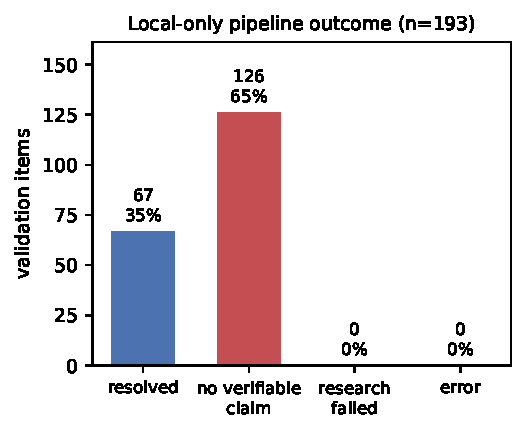
\includegraphics[width=0.92\linewidth]{figures/fig9_local_eval_outcomes.pdf}
\caption{Pipeline outcome for all 193 \texttt{validation} items,
local-only configuration. The \texttt{no\_verifiable\_claims} slice --
posts from which the local 3B model extracts nothing checkable -- is
almost twice the size of the slice that reaches a verdict.}
\label{fig:tl202outcomes}
\end{figure}

\paragraph{The binding constraint is claim extraction, upstream of everything else}
The 0\% research-failure rate rules out the search backend. The
per-class picture (Table~\ref{tab:tl202perclass},
Fig.~\ref{fig:tl202perclass}) localises the rest: \texttt{FALSE} --
83\% of the corpus -- is recovered with precision 0.80 but recall only
0.21; the model is accurate \emph{when} it commits to \texttt{FALSE},
but commits rarely. \texttt{MISLEADING} is \textbf{never once recovered
(0/7)}: the local model has no working notion of the ``authentic
material, false framing'' category that is the dominant real-world
pattern (80\% of the corpus is provenance-type). We inspected each of the 11
resolved items where a \texttt{FALSE}/\texttt{MISLEADING} claim received
an affirmative (\texttt{TRUE}/\texttt{MOSTLY\_TRUE}) verdict, comparing
the claim the pipeline actually verdicted against the item's recorded
ground-truth claim. \textbf{Nine of the 11 share the same root cause as
the abstentions}: the ``claim'' the model extracted was a fragment of
on-screen dialogue, a true incidental side-fact (``Rekha Gupta is the CM
of Delhi''), a recitation of a fixed text (the US Pledge of Allegiance),
or the fact-check's own correction rather than the post's assertion --
the pipeline then correctly verified a trivially-true fragment, a
claim-\emph{coverage} failure (Section~\ref{sec:multimodalanalysis}).
\textbf{The remaining two are genuine verdict-stage failures}: item-0116
(``India has brought down 2 Pakistani Fighter Jets'') and item-0111
(``India is now the fourth-largest economy in the world'') were faithful
restatements of the post's own assertion, extracted correctly and then
mis-verdicted \texttt{TRUE}/\texttt{MOSTLY\_TRUE} against a
\texttt{FALSE}/\texttt{MISLEADING} ground truth. Coverage dominates this
error class, but it does not exhaust it. This split is one reviewer's
item-level judgment on 11 cases and is reported as such.

\begin{table}[!t]
\caption{Per-class performance on resolved items ($n=67$). Classes with zero support and zero predictions omitted.}
\label{tab:tl202perclass}
\centering
\footnotesize
\begin{tabular}{@{}lrrrr@{}}
\toprule
Class & Precision & Recall & F1 & Support \\
\midrule
\texttt{FALSE}      & 0.80 & 0.21 & 0.33 & 57 \\
\texttt{MISLEADING} & 0.00 & 0.00 & 0.00 & 7 \\
\texttt{TRUE}       & 0.20 & 0.33 & 0.25 & 3 \\
\midrule
\multicolumn{4}{@{}l}{Macro-F1 (unweighted over the 3 classes)} & 0.194 \\
\bottomrule
\end{tabular}
\end{table}

\begin{table}[!t]
\caption{Confusion matrix, resolved items ($n=67$), ground-truth bucket $\times$ predicted bucket.}
\label{tab:tl202confusion}
\centering
\footnotesize
\begin{tabular}{@{}lrrrr@{}}
\toprule
GT $\downarrow$ / Pred $\rightarrow$ & \texttt{FALSE} & \texttt{MISL.} & \texttt{TRUE} & \texttt{UNVER.} \\
\midrule
\texttt{FALSE} ($n=57$)      & \textbf{19} & 1 & 10 & 27 \\
\texttt{MISLEADING} ($n=7$)  & 4 & \textbf{0} & 1 & 2 \\
\texttt{TRUE} ($n=3$)        & 1 & 1 & \textbf{1} & 0 \\
\bottomrule
\end{tabular}
\end{table}

\begin{figure}[!t]
\centering
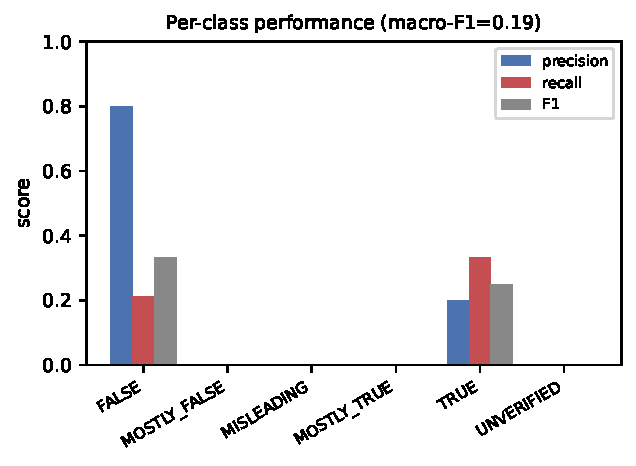
\includegraphics[width=0.92\linewidth]{figures/fig11_local_eval_perclass_f1.pdf}
\caption{Per-class precision, recall, and F1 on the 67 resolved
\textsc{TruthLens-202} items. \texttt{FALSE} carries the only non-trivial
signal, and even there recall is 0.21; \texttt{MISLEADING} is a total
miss.}
\label{fig:tl202perclass}
\end{figure}

\paragraph{Breakdowns}
Accuracy on resolved items does not move meaningfully with the corpus's
known skews. By platform: Facebook 4/7, X 15/54 (27.8\%), Instagram
1/6. By language: English 30.2\% (16/53), Hindi 33.3\% (4/12), Bengali
0/2. By ground-truth label: \texttt{FALSE} 33.3\% (19/57),
\texttt{MISLEADING} 0/7, \texttt{TRUE} 1/3. Crucially, the 78 items
that \emph{did} carry a backfilled vision context scored no better
(27.6\%, 8/29 resolved) than the 115 without it (31.6\%, 12/38) --
consistent with the pre-registered concern that \texttt{llava-phi3} on
compressed social-video keyframes adds little, and evidence that the
deferred visual analysis (Section~\ref{sec:truthlens202}, limitation 4)
is not the missing piece here.

\paragraph{What this is, and is not}
This is a first-run, single-configuration floor on a
deliberately-skewed, single-annotator corpus; it is not a bound on the
architecture. It establishes three things concretely: (i) with a local
3B model, \emph{claim extraction} -- not retrieval -- is the component
that determines whether short-form political misinformation gets checked
at all, and it fails on roughly two-thirds of real posts, with verdict
reasoning a second, smaller failure surface on those that do resolve
(2 of 11 affirmative-verdicts-on-false; \texttt{MISLEADING} 0/7); (ii) the deterministic safeguards hold up
where they run (0\% research-failure, high \texttt{FALSE} precision, no
crash across 193 items); (iii) the \texttt{MISLEADING}/provenance
category needs explicit modelling that the current text-only extraction
does not provide. Section~\ref{sec:futurework} lists the configurations
(larger local model, a vision-first extraction path, a metered cloud
escalation tier) whose evaluation against this same held-out split is
now the open work.

\section{Ablation Study}
\label{sec:ablation}

Three analyses are in scope for this program (Section
\ref{sec:expmethodology}); this section reports the claim-decomposition
counterfactual in full and summarizes the other two, cross-referencing
their detailed writeups.

\subsection{Claim-decomposition counterfactual (single-claim vs.\ multi-claim), $n=4$}
\label{sec:decompcounterfactual}
This is a \emph{counterfactual reanalysis of already-collected verdict
data}, not a freshly-run paired experiment, and we name it that way
rather than call it a clean ablation: each real claim's verdict is an
independently computed research-then-reasoning result regardless of how
many total claims were extracted in that run, so reusing the real
per-claim verdict to ask "what would aggregating only the primary claim,
vs.\ all claims, produce" is a valid way to isolate the
\emph{aggregation} mechanism's effect. It is \emph{not} a test of
whether decomposing in the first place changes upstream search or
evidence-gathering behavior for the primary claim -- that would require
an independently-run single-claim-only pipeline configuration, which
does not exist. No new LLM calls were made; restricted to the 4 items
with more than one verifiable claim, since aggregation is a no-op on a
single-claim item by construction.

\begin{table}[!t]
\caption{Claim-decomposition ablation}
\label{tab:decomposition}
\centering
\footnotesize
\begin{tabular}{lrrr}
\toprule
Condition & $n$ & Correct & Accuracy \\
\midrule
Single-claim (primary only) & 4 & 1 & 25.0\% \\
Multi-claim (full decomposition) & 4 & 2 & 50.0\% \\
\bottomrule
\end{tabular}
\end{table}

\begin{table*}[!t]
\caption{Per-item detail (\ding{51} = correct, \ding{55} = wrong)}
\label{tab:decomposition-detail}
\centering
\footnotesize
\begin{tabular}{lccc}
\toprule
Item & Single-claim result & Multi-claim result & Ground truth \\
\midrule
item-0001 & \ding{55}\ UNVERIFIED & \ding{51}\ MOSTLY\_FALSE & FALSE \\
item-0002 & \ding{51}\ MOSTLY\_FALSE & \ding{51}\ MOSTLY\_FALSE & FALSE \\
item-0004 & \ding{55}\ FALSE & \ding{55}\ FALSE (no-op, 1 claim) & TRUE \\
item-0005 & \ding{55}\ FALSE & \ding{55}\ FALSE & MISLEADING \\
\bottomrule
\end{tabular}
\end{table*}

\begin{figure}[!t]
\centering
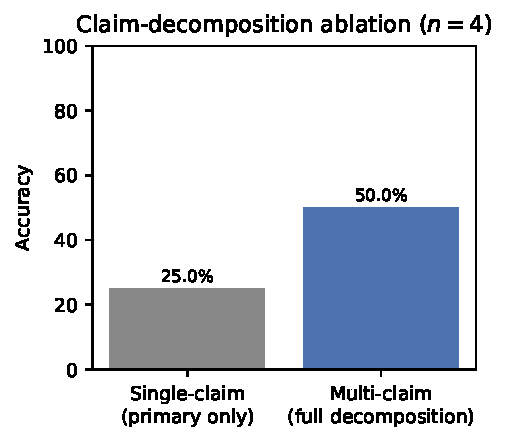
\includegraphics[width=0.85\linewidth]{figures/fig3_decomposition_ablation.pdf}
\caption{Table~\ref{tab:decomposition} plotted. A counterfactual
reanalysis, not an independently-run ablation (Section
\ref{sec:decompcounterfactual}), isolating deterministic aggregation as a
real contributor once claim extraction has more than one claim to work
with.}
\label{fig:decomposition}
\end{figure}

This is a real, positive result for RQ2's decomposition-specific question,
about the \emph{aggregation} mechanism specifically. On item-0001, the
single highest-importance claim landed on \texttt{UNVERIFIED} (a
missing-citation validator downgrade), but aggregating all 4 extracted
claims via the deterministic rule table (Section~\ref{sec:aggregation})
correctly recovered \texttt{MOSTLY\_FALSE}. $n=4$ is far too small to
generalize, but this is the clearest component-level evidence in this
program that aggregation helps rather than hurts once claim extraction
has more than one claim to work with, reported with the same prominence
as Section~\ref{sec:results}'s findings, not buried beneath them.

\subsection{Validation ablation (RQ1) -- summary}
Baseline 4 (TruthLens minus validation) is the primary ablation for RQ1;
its result is the unsupported-output-rate comparison in
Section~\ref{sec:evidencevalidation} (66.7\% without validation vs.\ 55.6\%
with it, on the original 9-case validator audit, before the two general
fixes reported in the same section improved that further).

\subsection{Source-tier ablation (RQ4) -- summary}
Restricting research-planning queries explicitly targeting primary sources
to a fixed government/legal domain allow-list, versus the system's normal
unrestricted queries, is evaluated in full in Appendix~\ref{sec:appendixevidence}
(summarized in Section~\ref{sec:evidencevalidation}):
tier-classification rate moved from $\sim$11\% to 95\% under restriction,
measured on a different, smaller query sample than the system's normal
operating condition, with a disclosed residual gap in full-text fetch
reliability specific to \texttt{.gov.in} domains.

\section{Evidence and Validation Analysis}
\label{sec:evidencevalidation}

\subsection{Validator methodology}
The real production pipeline was run with \texttt{SKIP\_VALIDATION=True}
so the raw proposal is always persisted, while
\texttt{validate\_verdict()}'s outcome is still always computed --
giving both the WITHOUT- and WITH-validation view from one real LLM call
per claim. 9 verifiable claims resolved across 4 items (0001, 0002, 0004,
0005); items 0006/0007 had zero verifiable claims (Section
\ref{sec:multimodalanalysis}). Ground truth is a single, unadjudicated
draft human review -- every number below is directional pending
independent review. One real bug was found and fixed mid-audit: a
single-bracket citation's UUID hex fragments leaked through the
number-grounding check as apparent unsupported statistics (item-0004),
fixed by stripping anything UUID-shaped independent of bracket style --
with a disclosed side effect (it removed an accidental protection that
had been shielding a \emph{substantively wrong} verdict, Section
\ref{sec:failuremodes}).

\subsection{Original confusion matrix ($n=9$, single unadjudicated reviewer)}
\begin{table}[!t]
\caption{Validator confusion matrix, before the two general fixes below}
\label{tab:validator-before}
\centering
\scriptsize
\begin{tabular}{lcc}
\toprule
 & Validator downgrades & Validator passes \\
\midrule
Human: unsupported & 1 (TP) & 5 (FN) \\
Human: fine to publish & 0 (FP) & 3 (TN) \\
\bottomrule
\end{tabular}
\end{table}

Caveat: 3 of the 4 recorded downgrades are ``no-op'' -- the raw proposal
was already \texttt{UNVERIFIED} with an empty citation list, so the
check fires trivially without changing the published label. Counted as
TN (nothing wrong was going to publish either way), not a meaningful
catch -- some unknown share of any raw ``X\% downgraded'' number may be
this kind of no-op.

\textbf{Validator Precision} = 1/1 = 100\% (Wilson 95\% CI: 20.7--100\%).
\textbf{Validator Recall} = 1/6 = 16.7\% (Wilson 95\% CI: 3.0--56.4\%).
\textbf{Validator F1} $\approx$ 28.6\%.

\subsection{Unsupported output rate, and why recall is low}
Of the 9 raw proposals, 6/9 (66.7\%) are judged, by draft human review,
unsupported enough that publishing them as-is would mislead -- wrong
-entity evidence treated as contradicting; a label contradicting the
reasoning's own ``no reliable information'' conclusion; two confident
labels contradicting independent Tier-1 ground truth. The original three
checks catch only 1 of these 6. \textbf{Unsupported output rate WITHOUT
validation: 6/9 (66.7\%). WITH validation: 5/9 (55.6\%)} -- real and
positive, more modest than a raw downgrade rate alone would suggest.
Every one of the 5 false negatives fails for a reason citation existence,
source-fetch existence, and numeric grounding structurally cannot detect:
label/reasoning inconsistency (motivated the new Check 4, below);
wrong-entity evidence treated as relevant; vague reasoning that still
clears a word-count bar; and a verdict simply, factually wrong relative
to ground truth that no citation check can catch if the model misweighs
real, present evidence.

\subsection{Addendum: re-scoring after two general fixes, with a circularity caveat}
Two general, deterministic fixes were added to \texttt{validate\_verdict()}
after the headline finding in Section~\ref{sec:results}: the UUID-leak
fix above, and the new label/reasoning-consistency check
(Section~\ref{sec:validation}) -- both pure functions of the model's own
output, never of ground truth, so re-scoring the same 9 cases costs no
new LLM calls and is not answer-tuning.

\begin{table}[!t]
\caption{Validator confusion matrix, after the two general fixes}
\label{tab:validator-after}
\centering
\scriptsize
\begin{tabular}{lcc}
\toprule
 & Validator downgrades & Validator passes \\
\midrule
Human: unsupported & 2 (TP) & 3 (FN) \\
Human: fine to publish & 0 (FP) & 4 (TN, all no-op) \\
\bottomrule
\end{tabular}
\end{table}

\begin{figure}[!t]
\centering
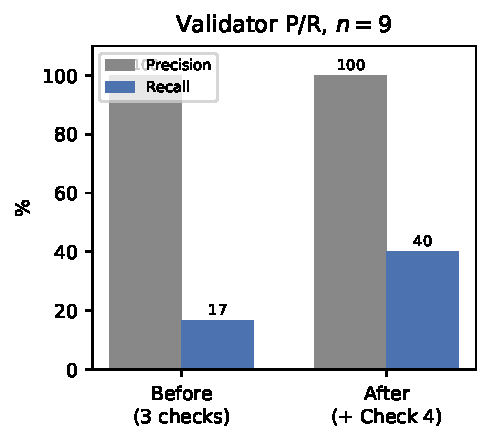
\includegraphics[width=0.85\linewidth]{figures/fig4_validator_before_after.pdf}
\caption{Validator precision/recall before vs.\ after the two
general fixes (Tables~\ref{tab:validator-before} and
\ref{tab:validator-after}, $n=9$). Precision holds at 100\%; recall
improves 16.7\%$\to$40\% -- with the calibration circularity disclosed
in the text.}
\label{fig:validator}
\end{figure}

\textbf{Precision 100\% (2/2), Recall 40\% (2/5)} -- up from 16.7\%. The
two new true positives are the two most consequential original false
negatives, including a confident \texttt{FALSE} at confidence 0.8 that
contradicted independent Tier-1 ground truth, now correctly downgraded.
\textbf{A real regression, reported with equal prominence:} the audit's
one original true positive is no longer downgraded, since the UUID-leak
fix removed the false trigger that had been \emph{accidentally} catching
it -- the underlying wrong-entity problem remains genuinely uncaught;
net effect 1 TP lost, 2 gained, landing at 2 TP / 5 FN.

\textbf{A disclosed circularity, now tested rather than left as a
suspicion:} the new check's phrase list was written after reading the
two cases it now catches, so 40\% is likely optimistic about
generalization. Four real paraphrases never in the original phrase list
were each tested against a confident label in a synthetic evidence
matrix (\texttt{VALIDATOR\_SYNTHETIC\_BENCHMARK.md}, full phrasings in
Appendix~\ref{sec:appendixevidence}); \textbf{all four were missed} --
Check 4 does not generalize beyond its literal phrase list, confirming
the threat to validity already disclosed (Section~\ref{sec:threats}).

\textbf{Reel-level accuracy did not change (2/6) despite this real
validator improvement} -- itself a finding, not a disappointment to
explain away (Section~\ref{sec:discussion}).

\subsection{Evidence quality (RQ4): tier, stance, and diversity distribution ($n=68$ sources, 9 claims)}
\begin{table}[!t]
\caption{Source tier distribution ($n=68$)}
\label{tab:tiers}
\centering
\footnotesize
\begin{tabular}{lrr}
\toprule
Tier & Count & \% \\
\midrule
other & 43 & 63.2 \\
primary\_government & 14 & 20.6 \\
established\_news & 6 & 8.8 \\
primary\_legal & 2 & 2.9 \\
news\_wire & 2 & 2.9 \\
factcheck\_org & 1 & 1.5 \\
primary\_data & 0 & 0.0 \\
\bottomrule
\end{tabular}
\end{table}

Source-tier classification rate (primary tiers combined): 16/68 = 23.5\%
(Wilson 95\% CI: 15.0--34.9\%) on this sample's normal, unrestricted
queries -- a different experimental condition from the domain-restricted
result below, not a contradiction.

\begin{table}[!t]
\caption{Evidence stance distribution ($n=68$)}
\label{tab:stance}
\centering
\footnotesize
\begin{tabular}{lrr}
\toprule
Stance & Count & \% \\
\midrule
irrelevant & 58 & 85.3 \\
contradicts & 8 & 11.8 \\
supports & 2 & 2.9 \\
provides\_context & 0 & 0.0 \\
\bottomrule
\end{tabular}
\end{table}

85.3\% of retrieved-and-analyzed sources were judged irrelevant --
notably higher than an earlier, smaller development-time figure of
55.6\%, both real and reported since this ratio moves across samples.
Source diversity: 29 distinct domains across 68 sources.

\subsection{The four-way primary-source metric, not collapsed into one number}
Four distinct, independently reported metrics, not one collapsed number
(full per-metric breakdown and illustrative wrong-domain/wrong-country
examples: Appendix~\ref{sec:appendixevidence}): \textbf{(1) source-tier
classification rate} 16/68 = 23.5\%; \textbf{(2) relevant primary source
rate} (draft human judgment) 11/16 = 68.75\%; \textbf{(3) primary source
fetch-success rate} 16/16, by construction of an existing fetch
guarantee; \textbf{(4) usable evidence extraction rate} 3/16 = 18.75\%
(stance $\neq$ \texttt{irrelevant}).

\begin{figure}[!t]
\centering
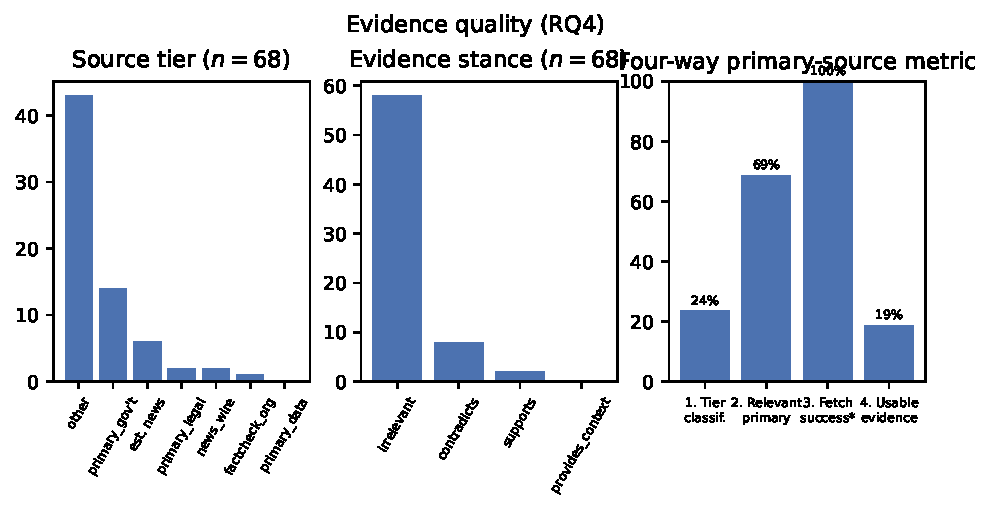
\includegraphics[width=\linewidth]{figures/fig5_evidence_quality.pdf}
\caption{Source-tier distribution, evidence-stance distribution,
and the four-way primary-source metric ($n=68$ sources, 9 claims).
$^*$Metric 3 holds by construction of an existing fetch guarantee, not
independently re-measured this pass.}
\label{fig:evidencequality}
\end{figure}

\textbf{The gap between metric 2 (68.75\%) and metric 4 (18.75\%) is the
single most important finding of this evaluation.} Retrieval finds real,
topically-appropriate primary sources at a meaningfully higher rate than
the usable-evidence number would suggest -- the bottleneck is that most
of these sources are homepages or generically-relevant documents too
broad to confirm one specific atomic fact, not a failure to find
relevant sources. Metric 4 alone would read as poor retrieval quality;
both metrics together show the more accurate picture.

\subsection{A second major bug, a search-side fix, and an unintegrated
entity-consistency prototype}
Three further findings from this same evidence-quality audit are
reported in full in Appendix~\ref{sec:appendixevidence}, summarized
here: (1) 32/68 (47.1\%) real evidence rows had an empty
\texttt{explanation} field despite a valid stance label -- the same
schema-valid-but-empty class found elsewhere, never guarded at this
stage, fixed with a per-source substantiveness check
(Section~\ref{sec:cascade}); (2) restricting primary-source-targeting
queries to a fixed government/legal domain allow-list, rather than
trusting a model-written \texttt{site:gov.in}, moved tier-classification
from $\sim$11\% to 95\% on seven re-run queries, with a disclosed
residual \texttt{.gov.in} full-page-fetch reliability gap; (3) a
prototype entity-consistency check (does a claim's extracted entity
appear in its cited evidence?) found one genuine true positive on the
real 9-claim sample -- refining item-0004's error attribution to a
concrete evidence mismatch (Burdwan, West Bengal vs.\ Delhi Police) --
alongside diagnosed false-positive causes, and is explicitly
\textbf{not integrated into production}: too small a sample to justify a
fifth check without more data (Rule 4).

\section{Multimodal and Visual Failure Analysis}
\label{sec:multimodalanalysis}

\subsection{Defining claim coverage}
\label{sec:claimcoveragedef}
Every use of ``claim coverage'' means one operationalized judgment: a
benchmark claim is \textbf{covered} when at least one extracted claim
identifies the same factual proposition as the professional fact-check's
own claim -- matching on subject/entity, event, predicate, and any
temporally-relevant qualifier -- judged by a human annotator blind to
which pipeline configuration produced the extraction (\texttt{METRICS.md}
\S2). Topical overlap alone does not count. This is necessarily a human
judgment, not a string-similarity score, since paraphrase makes automated
matching unreliable at this scale; every pairwise judgment is recorded in
\texttt{research/claim\_coverage\_results.csv} for audit.

\subsection{What was run}
Real ingestion of the 7-item dataset as it existed at the time, followed
by claim extraction under three input-modality conditions:
\texttt{text\_only}, \texttt{text\_ocr} (+ on-screen text),
\texttt{text\_ocr\_vision} (+ vision-context description) -- all
local-model-only, isolating the modality variable the same way the
baselines isolate architecture. TruthLens has exactly three input
signals feeding claim extraction, so \texttt{text\_ocr\_vision}
\emph{is} full multimodal for this system. Ingestion: 6 of 7 items
usable -- item-0003 failed both attempts (persistent Instagram-side
error); item-0005 initially failed on a differently-phrased yt-dlp ``no
video'' message, fixed and re-verified live
(Section~\ref{sec:failuremodes}).

\subsection{Claim coverage results ($n=6$, item-0003 excluded)}
\begin{table}[!t]
\caption{Claim coverage by input modality}
\label{tab:coverage}
\centering
\scriptsize
\begin{tabular}{lrrl}
\toprule
Condition & Covered & Coverage & 95\% CI \\
\midrule
text\_only & 1/6 & 16.7\% & [3.0,56.4] \\
text\_ocr & 0/6 & 0.0\% & [0.0,39.0] \\
text\_ocr\_vision (full) & 2/6 & 33.3\% & [9.7,70.0] \\
\bottomrule
\end{tabular}
\end{table}

\begin{figure}[!t]
\centering
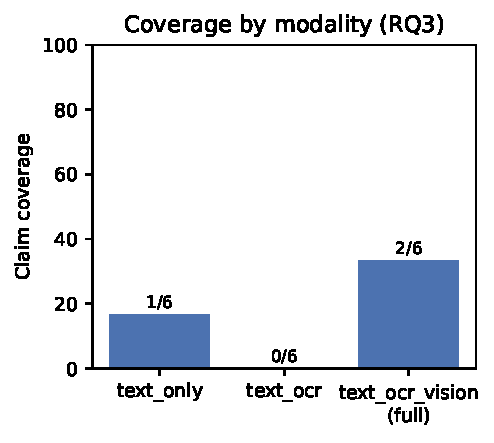
\includegraphics[width=0.85\linewidth]{figures/fig6_multimodal_coverage.pdf}
\caption{Table~\ref{tab:coverage} plotted. \texttt{text\_ocr}
scoring below \texttt{text\_only} is reported as a real result, not
suppressed (Section~\ref{sec:multimodalanalysis} explains the likely
cause).}
\label{fig:multimodal}
\end{figure}

Read these as exactly what they are: 6 single, non-repeated LLM calls per
condition, CIs wide enough to overlap almost entirely.
\texttt{text\_ocr} scoring below \texttt{text\_only} is real, reportable,
not suppressed for complicating the ``more modality is better''
hypothesis -- the likely (unverified) explanation is single-call noise
compounded by a specific extraction failure, not a robust modality
effect.

\subsection{item-0004: the one clean, positive RQ3 result}
The real transcript is badly garbled (chaotic protest audio); real OCR,
sampled across frames, clearly and repeatedly captured on-screen text
asserting the actual checkworthy claim (police using a nail-fitted baton),
matching the fact-check's own verdict almost verbatim.
\texttt{text\_only} extracted nothing resembling it; \texttt{text\_ocr}
happened to return one empty-text claim on this run; \texttt{text\_ocr\_vision}
correctly surfaced the claim, messily (7 near-duplicate claims, one per
noisy OCR-frame variant -- a new, unfixed failure mode, no existing check
evaluates cross-claim redundancy). Only the multimodal condition produced
any usable signal, via OCR content the audio transcript had no access to
-- a genuine, small-$n$ demonstration of what RQ3 asks about.

\subsection{The cross-post attribution problem}
\label{sec:crosspost}
Drafting atomic claims against the real ingested content surfaced a
structural pattern named explicitly here: the \textbf{cross-post
attribution problem}. The same underlying media $M$ can be published as
Post $A$ asserting claim $C$, and separately as Post $B$ asserting a
different claim $C'$ -- a system ingesting only one post URL cannot
discover the other claim from that post's own content at all.
\textbf{4 of 6 scoreable items} have their actual false claim living
entirely outside the specific post's own content, added by a different
account recirculating the same video under a new caption; only item-0004
(and partially item-0007) have the checkworthy claim actually on-screen
in the URL this dataset points to -- structural, not a sampling
accident, and TruthLens has no reverse-video/cross-post matching
capability. Full formalization and discussion of why this is structural
rather than incidental, and why we did not prototype a fix against this
program's own benchmark: Appendix~\ref{sec:appendixcrosspost}.

\subsection{New failure modes found this pass}
\textbf{Near-duplicate claims from noisy OCR-frame variants}
(item-0004, above), uncaught since no existing check evaluates
cross-claim redundancy. \textbf{\texttt{importance} values outside its
declared [0,1] range} causing schema-validation failure (item-0005:
$-1$, then a run of 2--6 resembling an ordinal position substituted for a
score) -- occurred only because this script removes the Gemini
-escalation cascade to isolate the modality variable, so production's
\texttt{FallbackLLMProvider} would likely mask this normally.
\textbf{The vision-output prompt-echo bug recurred 4 more times}
(items 0002, 0004, 0006; items 0001, 0007 produced empty vision output
instead) -- a repeated, frequent vision-stage failure, not a rare
anecdote, motivating the general fix in Section~\ref{sec:cascade}. Only
item-0005's vision output was genuinely coherent. This fix's real-world
impact on Section~\ref{sec:results}'s numbers is not independently
re-verified end-to-end (the paid fallback's quota was already exhausted
before it could be exercised against items 0006/0007, whose underlying
problems are not primarily vision-related, so no change is expected --
an expectation, not a verified result).

\section{Bias, Calibration, and Efficiency Analysis}
\label{sec:bce}

\subsection{Political bias (RQ5): attempted, blocked by data availability, deferred honestly}
No genuine matched pairs exist in the current 9-item dataset (same topic,
structure, evidence availability, and difficulty, varying only the
political actor named): BJP has the most items (3) of any actor, but none
are topic-matched against another single actor -- a disclosed
methodological choice trading this analysis away for broader dataset
coverage, not attempted as a quantitative result. Named as the top open
item for whoever continues this program (Section~\ref{sec:futurework}).
One qualitative data point (not a substitute for the real analysis,
full discussion: Appendix~\ref{sec:appendixbce}): the system was willing
to reach \texttt{FALSE} against a claim traceable to a government actor's
own public position (item-0004), a necessary but nowhere near sufficient
condition for what RQ5 actually asks.

\subsection{Calibration (RQ6): not computed, per our own pre-registered fallback rule}
Nine real confidence values exist: 0.0, 0.0, 0.1, 0.1, 0.2, 0.2, 0.2, 0.7,
0.8 -- too few per bin to meet our pre-registered calibration gate (no
bin under 3 items) no matter how bins are drawn, so per our protocol's
fallback rule, no ECE or Brier score is reported. One heavily caveated
observation on this raw distribution: Appendix~\ref{sec:appendixbce}.

\subsection{Efficiency}
\begin{table}[!t]
\caption{Efficiency, real measured data}
\label{tab:efficiency}
\centering
\scriptsize
\begin{tabular}{lccc}
\toprule
Config & LLM calls & Latency & Cost \\
\midrule
B2: Search+LLM & 1 & $\sim$15.9s & \$0 \\
B3: Search+RAG+LLM & 1 & $\sim$17.8s & \$0 \\
Full TruthLens & $\sim$9.6/claim$^\ddagger$ & n/m & \$0/paid mix \\
\bottomrule
\end{tabular}
\\[2pt]
\raggedright\footnotesize $^\ddagger$Derived from 7.56 sources/claim
(avg.), each requiring one evidence-analysis call, plus one
research-planning and one verdict call per claim. n/m = not measured in
this pass (disclosed gap, below).
\end{table}

\begin{figure}[!t]
\centering
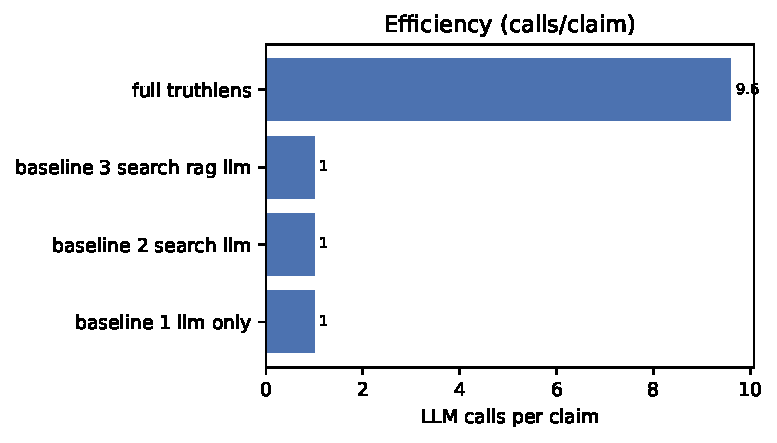
\includegraphics[width=0.9\linewidth]{figures/fig7_efficiency.pdf}
\caption{LLM calls per claim by configuration
(research/system\_efficiency.csv). Full TruthLens's call count is
derived from real average sources/claim, not directly measured
end-to-end; latency is not shown, a disclosed gap (text).}
\label{fig:efficiency}
\end{figure}

Full TruthLens is not directly latency-comparable to the two baselines --
a disclosed gap, since the validator-audit run did not capture per-claim
wall-clock time. What is measurable: full TruthLens's real cost/time per
claim is necessarily several times either baseline's from call count
alone -- roughly 9.6 LLM calls per claim against the baselines' fixed 1.
Full latency/cost gap detail: Appendix~\ref{sec:appendixbce}.

\section{Foundation-Phase System Extensions}
\label{sec:foundationphase}

A subsequent work program, run against a 13-phase research roadmap
(\texttt{research/RESEARCH\_ROADMAP\_V2.md}), extended the dataset and
system. \textbf{Scope discipline:} none of this re-measures reel-level
accuracy or touches the frozen six-item comparison
(Section~\ref{sec:results}); new benchmark items are held in a
\texttt{validation} split used for no tuning decision. Every number
traces to a versioned experiment (EXP-009--030,
\texttt{experiments/registry.jsonl}; full numbers
Appendix~\ref{sec:appendixfoundation}); negative and inconclusive
results are kept as prominent as positive ones.

\subsection{Dataset growth and two new validator checks}
\label{sec:newchecks}
Six new items from the same fact-checker pool (BOOM Live, Alt News),
each live-URL- and content-hash-checked, grew the set 9$\to$15
(12 FALSE / 2 MISLEADING / 1 TRUE -- still no second TRUE item after two
sourcing passes, consistent with the disclosed debunk-vs-confirmation
skew) and were assigned to a \texttt{validation} split.

Two checks were added to \texttt{validate\_verdict()} under the same
discipline as the original four (prototype, then integrate only once
real evaluation clears a stopping bar). \textbf{Check 6 (temporal
consistency)} flags a verdict when the claim asserts an explicit date
and every dated cited source predates it by $>2$ days -- deliberately
narrow, since real \texttt{time\_reference} values here are almost all
vague. \textbf{Check 7 (entity consistency)} flags a verdict when none
of the claim's PERSON/ORG/LOCATION entities appear (exact or fuzzy,
\texttt{SequenceMatcher} $\geq 0.75$ tuned on real transliteration
pairs) in a cited source whose stance influenced the verdict -- a
promotion of a previously-unintegrated prototype whose 4 false positives
(all one abstract-concept entity) motivated a type filter; the
corrected re-evaluation found 2/2 flagged violations genuine, zero
false positives. \textbf{Measured effect:} the adversarial synthetic
validator benchmark, expanded 28$\to$34 cases, moved precision
81.8\%$\to$87.5\% and recall 50.0\%$\to$60.9\%, and \emph{the
previously-named uncatchable entity-mismatch gap case is now caught};
the benchmark's only two false positives are the same pre-existing
Check-3 limitation, so both new checks add recall at zero measured
precision cost.

\subsection{A cross-cutting reliability finding, confirmed four times}
\label{sec:reliabilityfinding}
Four experiments, each targeting a different stage, independently
surfaced the same pattern: \textbf{raw un-retried local-model
(\texttt{llama3.2}) output on real content is substantively empty or
unusable a large fraction of the time}, and the existing
Gemini-escalation quality retries do more real work than a
pipeline-level pass/fail reading suggests. Claim \texttt{source\_quote}
population: 0 of 12 real claims across 8 items (EXP-012), reconfirmed at
0 of 90 across an 8-way modality sweep (EXP-016). Evidence-stance
explanations: 80\% (16/20) of raw judgments run without the
substantiveness-retry safeguard had an empty explanation on one side
(EXP-017). Adversarial stress testing: zero crashes across six cases,
but the one case needing a quality retry hit real Gemini quota
exhaustion from this program's own usage (EXP-020). None of these was
designed to measure model reliability; each surfaced it as a byproduct,
which is why four independent confirmations are more convincing than one
dedicated study.

\subsection{Retrieval, multimodal, and cross-post extensions}
\label{sec:foundationmultimodal}
\label{sec:foundationadversarial}
\textbf{Structured 5-query retrieval} (exact-claim, entity-focused,
primary-source, contradiction, context-history) raised source-tier
classification (23.5\%$\to$38.1\%, $n=42$ sources) but lowered
manually-judged relevance (68.75\%$\to$43.75\%) and usable-evidence
rate (18.75\%$\to$0\%) on this small sample -- traced to one claim with
no natural institutional subject receiving 7 of 16 primary-tier hits,
all irrelevant, because the primary-source query type fires
unconditionally; excluding it, the other three score 78\% relevant.
Reported as a mixed result, not smoothed into a win. \textbf{Full
8-combination multimodal re-analysis} reproduced rather than resolved
the original non-monotonic surprise: vision-alone highest on
ground-truth claim coverage (37.5\%), \texttt{ocr+vision} below every
single-signal condition (12.5\%). \textbf{Cross-post detection, stage 1
of 3}: a perceptual-hashing first-pass filter validated against real
re-extracted frames (same-video Hamming distance 0; different-video 20,
threshold 10); stages 2--3 not built. \textbf{Bounded adversarial stress
testing} of claim extraction (six hand-built cases) produced zero
crashes and no cross-signal hallucination, but surfaced two unnamed
gaps: no check tests caption/transcript mutual consistency, and
mixed-script content showed a possible Latin-script extraction bias.

\subsection{Two named gaps investigated}
\label{sec:followup}
The \textbf{input-signal consistency check} is infeasible in its cheap
form: caption-vs-transcript keyword (Jaccard) similarity, calibrated on
real data before shipping, is 0.000 for every legitimate benchmark item
checked ($n=4$) -- captions and transcripts are different registers,
often different languages, even when consistent. The
\textbf{multilingual-extraction bias} does \emph{not} generalize:
against the 90-claim dataset, non-Latin-script claims are the majority
(48/90) and script distribution tracks each item's dominant language,
including one genuinely code-switched item that produced both scripts.
The original single-case finding was real but narrow; \emph{we report
the correction as prominently as the finding}. The \texttt{source\_quote}
population gap was attacked with a strengthened extraction prompt (a
self-check procedure plus a worked example from a real miss): 0\%
population before and after ($n=8$), and on the example's own item the
strengthened prompt produced zero claims where the baseline produced
seven -- a clean negative result for prompt engineering as the fix.
Finally, the 6 VALIDATION items were run through the complete real
pipeline and committed: 4 produced zero claims, two produced 3 real
claims with real verdicts, and Check 7 correctly downgraded a
Jharkhand-police claim cited against an unrelated 2026 IIT Palakkad
article -- the first live confirmation it generalizes to new production
data.

\subsection{A second pass: aggregation, a security defense, a verdict-stage gap}
\label{sec:secondpass}
\textbf{Aggregation (Phase 10)} was unblocked by the population pass:
exactly one VALIDATION item (item-0010) qualified. Single-claim-only
missed (\texttt{UNVERIFIED} vs.\ ground truth \texttt{FALSE}); full
decomposition via the production \texttt{derive\_overall\_verdict()}
resolved correctly to \texttt{FALSE} -- directionally consistent with
the $n=4$ DEV result, reported at its real $n=1$. \textbf{Cross-post
stage 2} (claim-embedding clustering) is blocked by a confirmed
infrastructure gap: the local Ollama server was not started with
embedding support and no embedding model is pulled -- disclosed as a
concrete prerequisite, not worked around. \textbf{Prompt-injection
defense} had zero test coverage despite processing untrusted content on
every post. Code review found the delimiter convention never neutralized
literal delimiter tokens already in untrusted text -- a deterministic
bypass, closed by sanitizing before wrapping, verified both directions.
Of 5 live adversarial attempts against claim extraction, a blunt
override succeeded once (the injected false claim emitted verbatim as a
maximum-importance verifiable claim) -- the first real measurement of
this project's stated expectation that small local models resist in-band
instructions less reliably; a hardened prompt reduced this to 0/5.
Carried through the pipeline, the one success was independently resolved
by the downstream validator to a correct evidence-grounded \texttt{FALSE}
citing 12 real sources ($n=1$, an unusually well-evidenced test claim).
\textbf{A new verdict-stage failure}: constructed evidence with a
0.95-reliability government source supporting and a 0.20-reliability
uncited source contradicting produced no \texttt{TRUE}/\texttt{MOSTLY\_TRUE}
in 0 of 14 trials across two prompt versions -- some with reasoning that
named the weak source as unreliable yet did not act on it, one pairing a
wrong label with maximum confidence. An explicit reliability-weighting
prompt rule did not resolve it (0/7) -- a measured negative result; the
rule is kept as objectively-correct guidance, not claimed as a fix. A
deterministic check (cited-evidence reliability vs.\ verdict direction)
was then built and held to the Checks-6/7 bar -- 10/10 synthetic, 14/14
observed wrong trials caught, 0/34 benchmark interactions -- and
integrated as \textbf{Check 8} with precision/recall unchanged
(87.5\%/60.9\%). A direct re-run of the evidence-stance taxonomy
comparison fixed its own confound (porting in the substantiveness-retry
safeguard) but hit a hard external ceiling: a real HTTP 429 confirmed
the fallback model's free tier is capped at 20 requests/day, which this
program's usage repeatedly exhausts; three attempts (4/20, 6/20, 5/20
clean rows) remain inconclusive about the candidate taxonomy's value.

\subsection{A benchmark-scaling session: a measured structural yield ceiling}
\label{sec:massSourcing}
Manual sourcing (one article read and judged at a time) added three
items, 15$\to$18, at roughly one usable item per 20--30 articles --
consistent with the original $\sim$8\% estimate -- before its throughput
was judged too slow against an instruction to reach a several-hundred-item
benchmark. An automated pipeline replaced the human read-and-judge step
with a local \texttt{llama3.2} judge call (every other step kept as
code): given a fact-check article and a cited Instagram post's real
caption (fetched via \texttt{yt-dlp}, never inferred), the judge decides
whether the post's \emph{own} caption asserts the specific false claim,
as opposed to the far more common case -- the central methodological
lesson of this pass -- of a fact-checker citing an Instagram post as
evidence of the true original event while the false claim was posted
separately, often on X/Twitter.

Five fact-checker archives were crawled to exhaustion or a clear
negative: \texttt{altnews.in} (4{,}967 articles, 515 candidates judged,
2 promoted); \texttt{vishvasnews.com} (two passes -- the second after a
URL filter was found to silently exclude most fact-check content;
1{,}682 candidates, 1 promoted); \texttt{thequint.com}'s WebQoof
(English + Hindi editions after an identical filter-gap finding; 859
candidates, 1 promoted); \texttt{factcrescendo.com} (English, Tamil,
Marathi, Malayalam; 533 candidates, 0 promoted); \texttt{factly.in}
(1{,}000 articles sampled, zero Instagram references, dropped).
\texttt{newschecker.in} was excluded, unattempted, on a
\texttt{robots.txt} directive against this crawler's user-agent. Two
contributing sources were only found to be contributing after fixing a
real filter bug -- Vishvas filtered on \texttt{/viral/} when 856 of 979
sampled URLs contained \texttt{fact-check} under other sections; WebQoof
missed a separate \texttt{/hindi/webqoof/} edition -- and a
post-judgment consistency filter had been checking a generic note
instead of the judge's real reasoning, letting self-contradicting
judgments through until manual review caught it (fixed; caught four more
immediately).

\textbf{The measured result:} across roughly 3{,}600 real candidates
judged over five sources, 4 were promoted (items 19--22, each verified
against the article and the post's caption before promotion) -- a
blended yield on the order of one promotable item per 900 candidates,
an order of magnitude worse than the $\sim$8\% a smaller manual pass had
suggested, and consistent with the earlier finding that most of this
dataset's false claims live outside the Instagram post being
fact-checked. At this rate a several-hundred-item target is not
reachable through deeper automated crawling of the same source type
\emph{under the Instagram-only constraint} -- a structural property of
where this pattern gets posted, not an effort gap (full detail:
\texttt{research/MASS\_SOURCING\_V2.md}).

\textbf{This finding was acted on.} Because the ceiling was a property
of the platform restriction, a later pass relaxed it -- admitting
X/Twitter, Facebook, and Instagram -- and added a review-gated
annotation step (a single reviewer adjudicates each screened candidate
against the full fact-check article), growing the \texttt{validation}
split from 13 to 193 items (202 with the frozen \texttt{dev} set): the
\textsc{TruthLens-202} corpus (Section~\ref{sec:truthlens202}). That
corpus is then evaluated end-to-end once, in a \$0 local-only
configuration (Section~\ref{sec:tl202eval}), which surfaces its own
finding: the local 3B model fails to extract a checkable claim from
65.3\% of real posts, making claim extraction -- not retrieval -- the
binding constraint on coverage, with verdict reasoning a second, smaller
failure surface on the posts that do resolve. Its construction carries
disclosed limitations (LLM-performed annotation under author direction;
$\sim$88\% single-source ground truth; three domain-driven skews), all stated in
Section~\ref{sec:truthlens202}.

\section{A Taxonomy of Failure Modes Found in Live Testing}
\label{sec:failuremodes}

Running the full system against real content end-to-end -- both during
original development and during this evaluation program itself --
surfaced 24 specific, reproducible failure modes we believe are
under-documented in the automated fact-checking literature at this level
of implementation detail, because they only appear when a system is run
against real content rather than evaluated on a static benchmark. We
consider this taxonomy, and the general lesson that most of these
failures were discoverable only this way, to be as practically important
a contribution of this work as any single architectural component. The
full list, each entry with its fix, is given in
Appendix~\ref{sec:appendixtaxonomy}; six representative entries,
spanning production code, research tooling, security, and this
program's own benchmark construction:

\begin{itemize}
\item \textbf{Schema-valid, substantively empty output}, found
  independently in four different pipeline stages (claim extraction,
  content generation, verdict reasoning, evidence analysis) -- no schema
  validation catches it; only a content-level substantiveness check does
  (Section~\ref{sec:cascade}), and each stage needed its own.
\item \textbf{Entity confusion between similarly-named organizations}
  and the downstream failure it caused: a downgraded verdict's
  hallucinated free-text reasoning was still reused verbatim on a
  rendered slide, because downgrading forces only the label, not the
  text.
\item \textbf{Baseline architecture silently inheriting a rescue
  mechanism under evaluation} (Section~\ref{sec:expmethodology}) -- an
  early draft of Baselines 2--3 called the same provider factory every
  production stage uses, giving both baselines the exact failure-rescue
  mechanism TruthLens's own architecture was being evaluated for having.
\item \textbf{A table-generation script's printed output and its
  persisted JSON summary silently disagreed}, found while building this
  paper's own figures (\texttt{day8\_final\_tables.py} reused two
  variable names across three unrelated computations) -- the same
  failure class as the production-code entity-confusion entry above,
  found in this project's own research tooling instead.
\item \textbf{Six synthetic validator benchmark cases silently tested the
  wrong check} (Section~\ref{sec:validation}/Phase 4,
  \texttt{VALIDATOR\_SYNTHETIC\_BENCHMARK.md}) -- cases built to isolate
  Check 4 had no citation at all, so Check 1 fired first and Check 4 was
  never reached, caught only by reading \texttt{validation\_status} in
  the raw output rather than trusting the benchmark's own design.
\item \textbf{A blunt prompt-injection override got past claim
  extraction once in 5 live attempts}, producing the injected false
  claim verbatim as a verifiable, maximum-importance claim -- the first
  real measurement (not just a stated expectation) that this system's
  delimiter-based defense is imperfect against small local models,
  confirmed independently by the downstream validator resolving the
  same injected claim to a correct \texttt{FALSE} verdict when carried
  through the rest of the real pipeline.
\end{itemize}

\section{Threats to Validity}
\label{sec:threats}
Thirteen threats, stated here at the density needed to be checkable; full
reasoning for the first ten: Appendix~\ref{sec:appendixthreats}. The last
three concern the \textsc{TruthLens-202} corpus, its ground-truth
provenance, and its local-only evaluation, and are detailed in
Sections~\ref{sec:truthlens202} and \ref{sec:tl202eval}.

\begin{itemize}
\item \textbf{Small, non-independent sample.} $n=9$ (6 resolved from
  every configuration), below this program's own 20--30 target; several
  proportions, including the headline 33.3\% accuracy figure, have
  Wilson intervals wide enough to be consistent with a different true
  rate.
\item \textbf{Single domain, single-country content.} Indian political
  short-form video only; source-tiering and prompts untested elsewhere.
\item \textbf{Single annotator, no inter-annotator agreement} on every
  draft judgment underlying Sections~\ref{sec:evidencevalidation}/
  \ref{sec:multimodalanalysis} (Tier-1 headline verdicts are exempt --
  they are independent organizations' own published verdicts).
\item \textbf{The new validator check's 40\% recall figure is measured
  on the same sample it was calibrated against} -- likely optimistic
  about generalization (Section~\ref{sec:evidencevalidation}).
\item \textbf{The vision-context fix's effect on headline accuracy is
  not independently re-verified} -- stated as an expectation, not a
  measured result.
\item \textbf{item-0003 is permanently excluded, not scored as a
  failure} -- confirmed unfetchable across three attempts.
\item \textbf{Baseline comparison isolates architecture from model, but
  not from claim-extraction coverage} -- Baselines 1--3 receive
  TruthLens's own already-extracted claim, so the headline comparison
  cannot fully separate architecture underperformance from claim
  -extraction giving it nothing to work with.
\item \textbf{The primary-source-retrieval fix is measured on tier
  classification, not full-text completeness}, on a distinct query
  sample; the \texttt{.gov.in} fetch-reliability gap it surfaced remains
  open.
\item \textbf{RQ5 and RQ6 are deferred by design, not omission}, per
  pre-registered fallback rules (Section~\ref{sec:bce}).
\item \textbf{Ground truth is sourced from a small set of professional
  fact-checkers whose editorial judgment we do not independently
  audit} -- a systematic coverage or resolution asymmetry would
  propagate undetected, since no second ground-truth source exists to
  check against.
\item \textbf{The evaluee screened its own test set.} The model that
  decided which of 11{,}544 candidates became \textsc{TruthLens-202}
  items (\texttt{llama3.2}) is the same model evaluated on the resulting
  corpus. The screen favours posts whose text that model can parse, so
  the selection bias runs toward easier items and the reported accuracy
  should be read as a favourably-selected floor
  (Section~\ref{sec:truthlens202}).
\item \textbf{\textsc{TruthLens-202}'s claim phrasing, label mapping and
  item selection were LLM-performed under author direction, not verified
  by a second human} (Section~\ref{sec:truthlens202}). Verdicts trace to
  an independent professional fact-check via a recorded verbatim quote,
  which bounds the risk, but the annotation layer is unaudited --
  a circularity concern given that an LLM-based system is the intended
  evaluee. The Section~\ref{sec:tl202eval} result is reported with this
  caveat attached and as a floor, not a validated headline; a
  second-annotator pass is the top open item
  (Section~\ref{sec:futurework}).
\item \textbf{\textsc{TruthLens-202} is $\sim$88\% single-source (Alt
  News) and carries three domain-driven skews} (83\% \texttt{FALSE},
  80\% X-sourced, 80\% \texttt{provenance}-type). The
  Section~\ref{sec:tl202eval} evaluation therefore leads with balanced
  accuracy and per-class F1, not raw accuracy, and treats the source
  concentration as a coverage limitation, not a representative sample
  of the fact-checking ecosystem.
\end{itemize}

\section{Discussion}
\label{sec:discussion}

\textbf{Audit your baselines as skeptically as your own system.} This
program's most consequential finding came not from improving TruthLens
but from a post-hoc audit that treated our own experimental design with
the skepticism this paper applies to the system under test, finding the
baselines quietly advantaged program-wide
(Section~\ref{sec:baselinefix}). Without it, this paper would have
published a confident, wrong-in-degree explanation for why TruthLens
loses to a single-shot baseline: the diagnosed causes (claim-extraction
coverage, validator false negatives) were real, but the uncorrected
number overstated their effect because part of it was an artefact of
unequal claim input. A baseline is part of the apparatus, not a neutral
reference, and deserves the same implementation-level scrutiny as the
system it is compared against.

\textbf{Label accuracy vs.\ support validity.} Two general,
ground-truth-independent fixes moved validator recall 16.7\%$\to$40\%
while reel-level accuracy stayed at 2/6, before and after the baseline
correction. \textbf{Label accuracy and support validity are different
axes that can move independently} -- a benchmark reporting only label
accuracy would have shown no progress during a pass that materially
reduced how often the system publishes a confidently wrong, unsupported
verdict.

\textbf{When TruthLens helps, specifically.} Once claim input is held
constant, full TruthLens beats two of three baselines and trails the
third by a much smaller margin; the two remaining wrong items are a
claim-extraction coverage failure (0006/0007) and one validator false
negative (0004). Table~\ref{tab:whenhelps} replaces a win/lose framing
with where the advantage materialises.
\begin{table}[!t]
\caption{Per-item conditions, corrected comparison ($n=6$)}
\label{tab:whenhelps}
\centering
\scriptsize
\setlength{\tabcolsep}{3.5pt}
\begin{tabular}{lccl}
\toprule
Item & Multi-claim? & Extracted? & TL vs.\ B2 \\
\midrule
item-0001 & Yes (4) & Yes & Both correct \\
item-0002 & Yes (2) & Yes & Both correct \\
item-0004 & No (1) & Yes & B2 only correct \\
item-0005 & Yes (2) & Yes & Both wrong \\
item-0006 & No (0) & \textbf{No} & Both wrong; TL abstains \\
item-0007 & No (0) & \textbf{No} & Both wrong; TL abstains \\
\bottomrule
\end{tabular}
\end{table}

Reading the matrix rather than the aggregate: TruthLens and Baseline 2
agree on every item where extraction succeeded and produced more than one
claim (0001, 0002) -- exactly where
Section~\ref{sec:decompcounterfactual}'s counterfactual shows aggregation
adding value. The one exclusive loss (0004) is single-claim, where
decomposition contributes nothing and the already-diagnosed validator
false negative costs it. Both systems fail identically when extraction
fails (0006/0007). Stated as a hypothesis for a larger dataset, not a
conclusion this $n$ supports: TruthLens's advantage over a single-shot
baseline may be concentrated in multi-claim items with successful
extraction and structurally absent where extraction fails or a post has
only one claim.

This tempers how DeVerna et al.'s finding
\cite{deverna2025curatedcontext} that curated context matters more than
reasoning ability should be read against ours: the corrected comparison
is broadly consistent with theirs -- TruthLens's curation-heavy
architecture is competitive with, and mostly ahead of, simpler
alternatives once claim input is fairly controlled -- but the lesson we
draw is methodological as much as architectural: curation-heavy systems
should be evaluated at the component level, with baselines audited as
carefully as the system, because an end-to-end label-accuracy number can
misattribute a claim-input confound to an architectural one. We did not
tune any prompt, threshold, or model choice on the frozen held-out set;
the validator fixes and the baseline correction are all
ground-truth-independent. We would rather report a real 33.3\%, a real
correction, and an honest account of both than a smoother number whose
provenance we could not defend.

\section{Future Work}
\label{sec:futurework}

Items already acted on in this program are marked; the rest are open.

\begin{enumerate}
\item \textbf{Evaluate \textsc{TruthLens-202} beyond the local-only floor}
  (\emph{corpus built and evaluated once}). Re-run the same 193-item
  held-out split under a larger local model, a vision-first
  claim-extraction path for provenance posts (where the visual \emph{is}
  the claim and text-only extraction fails on $\sim$65\% of items), and a
  metered cloud-escalation tier, reported together as a
  capability-vs.-cost ablation. This is the top result-bearing open item.
\item \textbf{A second, independent annotator} for the 165 review-gated
  \textsc{TruthLens-202} claim/label annotations (currently
  LLM-performed under author direction), a re-screen drawn from a
  different model family than the evaluee, and the Tier-2 draft
  judgments underlying
  Sections~\ref{sec:evidencevalidation}/\ref{sec:multimodalanalysis} --
  the prerequisite before the local-only result is a validated headline
  rather than a floor.
\item \textbf{Close claim-extraction coverage failures} on degraded
  audio and, more broadly, the near-zero verbatim \texttt{source\_quote}
  population (\emph{attacked}: a strengthened prompt did not move the
  rate, $n=8$; a structural change such as eliciting the quote before the
  claim is the next candidate). EXP-016 re-confirmed the degraded-audio
  gap across all 8 modality combinations.
\item \textbf{Video-provenance / cross-post verification}
  (\emph{stage 1 built}: a perceptual-hash first-pass filter validated on
  real frames). Stage 2 (claim-embedding clustering) is blocked by a
  confirmed infrastructure gap -- the local Ollama server lacks embedding
  support and no embedding model is pulled; stage 3 and pipeline
  integration are undone.
\item \textbf{Matched-pair sourcing for RQ5 and a large-enough set for
  RQ6}: both remain deferred by pre-registered rule -- RQ5 needs a
  sourcing pass matched on topic/structure/difficulty across political
  actors; RQ6's binning gate (no bin under 3 items) is unmet.
\item \textbf{Independently validate the deterministic checks} against
  phrasings and real production disagreement cases they were not
  calibrated on -- Checks 6/7/8 were held to a synthetic bar; the
  original four checks' circularity is still open, as is the
  \texttt{.gov.in} full-page-fetch reliability gap (403s, TLS failures).
\item \textbf{Extend the adversarial suite} to the categories needing
  real AI-generated-image, edited-video, and audio-corruption content
  (prompt-injection and contradictory-sources are now covered).
\item \textbf{Isolated test infrastructure for quota-dependent tests}:
  the collision between real concurrent Gemini usage and mocked scenarios
  is quantified (a confirmed 20-requests/day cap) but not fixed, and the
  live publishing-account connection and everything downstream of it
  remain unattempted.
\end{enumerate}

\section{Conclusion}
\label{sec:conclusion}

This paper reports the first evaluation of TruthLens against independent,
held-out ground truth, and leads with the least flattering result it
produced -- one in our own experimental design, not the system. A
skeptical post-hoc audit found our baselines had been given a cleaner
claim input than TruthLens's own extraction ever produced, program-wide,
contradicting our stated methodology and inflating baseline performance;
a research program that audits the system under test but never its own
baselines is not applying its standard uniformly. Corrected, full
TruthLens beats two of three baselines outright and trails the third by a
substantially smaller margin on the paired six-item sample, with the
residual gap tracing to claim-extraction coverage failures on two items
and one validator false negative -- more useful than the original
partly-artifactual negative number or an uncritical positive one. A
claim-decomposition counterfactual ($n=4$) separately shows aggregation
delivering a real gain (50.0\% vs.\ 25.0\%) once extraction produces more
than one claim, and two ground-truth-independent validator fixes moved
recall 16.7\%$\to$40\% (100\% precision) while leaving reel-level accuracy
unchanged -- a concrete demonstration that label accuracy and the
formally-defined \emph{support validity} construct are separable
properties. RQ5 (bias) and RQ6 (calibration) are deferred, not forced,
per pre-registered rules. The 24-entry taxonomy of failure modes
(Appendix~\ref{sec:appendixtaxonomy}) -- over a third found during this
evaluation, all but three paired with a deterministic check and a
regression test -- is as practically useful as any single number, since
most, including the baseline confound, are discoverable only by running a
complete system against real content.

A subsequent foundation-phase program
(Section~\ref{sec:foundationphase}) extends this without touching the
frozen comparison: the set grew to 15 items; two deterministic validator
checks (temporal, entity), each integrated only after clearing an
evaluation bar, moved adversarial-benchmark precision/recall
81.8\%/50.0\%$\to$87.5\%/60.9\% and closed a previously-named gap case;
four independent experiments converged on the same finding -- raw
local-model output on real content is substantively empty or unusable a
large fraction of the time, and the escalation defenses carry more of the
reliability burden than a pass/fail reading suggests. A prompt-injection
defense with zero prior test coverage was measured live (1/5 succeeded,
0/5 after a hardened prompt plus a deterministic delimiter fix, with the
downstream validator independently neutralising the one success), and a
genuinely new verdict-stage failure -- label selection not weighting
source reliability under contradiction (0/14 trials) -- was reported
unresolved after an insufficient prompt fix, then addressed with a
deterministic Check 8. A benchmark-scaling session measured a structural
ceiling: roughly one promotable item per 900 candidates under an
Instagram-only constraint, an order of magnitude below the initial
estimate, because most of this pattern's false claims are posted
elsewhere (often X/Twitter) than the fact-checked Instagram post.

Acting on that ceiling, a later pass relaxed the platform scope and added
a review-gated annotation step, producing \textsc{TruthLens-202} (193
\texttt{validation} items), and we run the full pipeline over all 193
once in a \$0 local-only configuration (Section~\ref{sec:tl202eval}),
reported as a floor with its limitations stated rather than softened:
34.7\% of posts reach a verdict, bucketed accuracy on those is 29.9\%
(below an always-\texttt{FALSE} baseline on balanced accuracy), the
annotation layer -- claim phrasing, label mapping and item selection --
was LLM-performed under author direction pending a second annotator, the
screening model was the same one later evaluated, and the corpus carries
a single-source majority and three domain-driven skews. Its one firm, transferable finding is diagnostic:
with a local 3B model, \emph{claim extraction} -- not retrieval (0\%
infrastructure failure) -- determines whether short-form political
misinformation gets checked at all, and it fails on roughly two-thirds
of real posts; verdict reasoning is a second, smaller failure surface on
those that do resolve. Work is paused here; the immediate
open items are the larger-local-model / vision-first / metered-cloud
ablation on the same held-out split, a second independent annotator, and
a broader ground-truth base (Section~\ref{sec:futurework}), alongside the
still-deferred RQ5/RQ6, the cross-post attribution problem, and the live
publishing-account connection -- none hidden in the sections above.

\appendix

\section{Extended Architecture Detail: Cascading and Aggregation}
\label{sec:appendixarchitecture}
Section~\ref{sec:cascade} summarizes verification-gated model cascading;
full detail follows. Five stages -- claim extraction, evidence analysis,
vision-context, content generation, and verdict proposal -- each run a
deterministic \emph{substantiveness check} before accepting local-model
output: claim extraction requires at least half of extracted verifiable
claims to have a \texttt{source\_quote} substring-grounded in the
transcript/OCR, and at least one claim with non-empty text (zero claims
is a legitimate ``found nothing,'' not a failure); evidence analysis
requires a non-empty per-source \texttt{explanation} (firing per-source
since this stage calls the LLM per source); vision-context checks
\texttt{scene\_description}'s word-overlap against the system prompt (the
0.20 threshold from Section~\ref{sec:cascade}); content
generation/verdict reasoning requires at least six real words after
stripping citation markup. On failure, the call retries once against a
paid model (Gemini) with an identical prompt, logged either way.
Illustrative development-time telemetry (predating the frozen evaluation,
not part of it) found this gate firing on 3/7 claim-extraction, 2/5
content-generation, and 2/8 verdict-proposal completions -- small counts,
large enough to show it firing routinely.

Section~\ref{sec:aggregation} summarizes deterministic aggregation and
grounded corrections; full detail follows. The reel-level rule table:
all \texttt{TRUE} yields overall \texttt{TRUE}; a mix of
\texttt{TRUE}/\texttt{MOSTLY\_TRUE} and \texttt{FALSE} yields
\texttt{MISLEADING}. Because a bare \texttt{FALSE}/\texttt{UNVERIFIED} is
a weak deliverable, the verdict-proposal call also carries optional
\texttt{corrected\_fact} and \texttt{context\_note} fields, held to the
same evidence-grounding rule as \texttt{reasoning\_summary}, left null
rather than guessed when unestablished. We deliberately did not build the
natural next step -- speculating about a claim's downstream consequences
-- since that is ungrounded generation of exactly the kind
Section~\ref{sec:validation} exists to prevent. Both fields are
invalidated whenever the parent verdict fails validation, even if
individually grounded.

\section{Extended Discussion: The Cross-Post Attribution Problem}
\label{sec:appendixcrosspost}
Section~\ref{sec:crosspost} defines the cross-post attribution problem
and states its headline number; full discussion follows. This is
structural, not a sampling accident: a fact-checker traces a viral claim
back to its original, differently-captioned source video, and that
video's URL is what enters the dataset (Section~\ref{sec:dataset}) -- a
majority of this dataset's items may be structurally unwinnable for
single-post claim extraction regardless of modality coverage. TruthLens
has no reverse-video/cross-post matching capability and has never
claimed one; we did not prototype a provenance-retrieval module against
this program's own benchmark, since evaluating it on the same 6 items
already read would violate our own held-out discipline -- a frozen,
disjoint pilot set is the correct next step (Section~\ref{sec:futurework}),
not attempted here.

\section{Threats to Validity: Full Reasoning}
\label{sec:appendixthreats}

Section~\ref{sec:threats} lists twelve threats at a checkable density;
the additional reasoning for the first ten follows in the same order (the
last two, on the \textsc{TruthLens-202} corpus and its local-only
evaluation, are detailed in Sections~\ref{sec:truthlens202} and
\ref{sec:tl202eval}).

\textbf{Small, non-independent sample.} $n=9$ (6 resolved from every
configuration) is far below this program's own 20--30 target and an ideal
50--100. Every proportion carries an exact count and a Wilson interval;
several, including the 33.3\% headline, have intervals wide enough to be
consistent with a different true rate.

\textbf{Single domain, single country.} Indian political short-form video
with English/Hindi/Urdu transcripts; source-tiering domain lists and
research-planning prompts are untuned and untested for other national
contexts.

\textbf{Single annotator, no IAA.} Every draft judgment in
Sections~\ref{sec:evidencevalidation}/\ref{sec:multimodalanalysis}
(validator TP/FP/TN/FN, evidence relevance, claim-coverage matching) is
one unadjudicated reviewer's; Tier-1 headline verdicts are exempt (they
are independent organisations' published verdicts).

\textbf{The new validator check's 40\% recall is measured on its own
calibration sample.} Likely optimistic for differently-phrased ``no
evidence found'' reasoning, since the phrase list was written after
reading the two cases it now catches; the principle is
ground-truth-independent, the implementation in this narrow sense is not.

\textbf{The vision-context fix's headline effect is not independently
re-verified} -- stated as an expectation (root causes of items 0006/0007
diagnosed as unrelated to vision quality), not a measured result; the
paid fallback's quota was exhausted before an end-to-end test.

\textbf{item-0003 is permanently excluded, not scored as a failure} --
confirmed unfetchable across three attempts, a real content-acquisition
limitation against Instagram, unaddressed by any fix here.

\textbf{The baseline comparison isolates architecture from model but not
from claim-extraction coverage.} Baselines 1--3 receive TruthLens's own
extracted claim, so the headline comparison cannot separate ``downstream
architecture underperforms'' from ``extraction gave it nothing for 2 of 6
items''; Section~\ref{sec:results} argues for the latter.

\textbf{The primary-source-retrieval fix is measured on tier
classification, not full-text completeness}, on a query sample distinct
from the main evidence-quality run; the \texttt{.gov.in} fetch gap it
surfaced (403s, TLS) is open.

\textbf{RQ5 and RQ6 are deferred by design}, per pre-registered fallback
rules (Section~\ref{sec:bce}), not reported with an underpowered number.

\textbf{Ground truth is a small set of professional fact-checkers whose
editorial judgment we do not independently audit.} Using their published
verdicts as Tier-1 truth is standard, but a systematic asymmetry in which
claims they cover or how they resolve ambiguity would propagate into
every number here undetected, with no second ground-truth source to
check against.

\section{Extended Bias, Calibration, and Efficiency Discussion}
\label{sec:appendixbce}
Section~\ref{sec:bce} states the headline RQ5/RQ6/efficiency facts; full
discussion follows.

\textbf{RQ5 qualitative observation, in full.} Of the 9 real verdicts
audited in Section~\ref{sec:evidencevalidation}, a verdict targeting a
government body's own claim (item-0004's Delhi Police baton case) was
treated no differently in kind by the pipeline than verdicts about party
or activist claims -- the system was willing to reach \texttt{FALSE}
against a claim traceable to a government actor's own public position (a
verdict itself judged wrong for reasons unrelated to which actor was
involved). One data point showing the system does not categorically
refuse to find against a government actor.

\textbf{RQ6 caveated observation, in full.} The two highest-confidence
verdicts (0.7, 0.8) are both cases Section~\ref{sec:evidencevalidation}'s
draft human review judged unreliable or factually wrong, while several
of the lowest-confidence verdicts (0.0--0.1) were appropriately cautious
\texttt{UNVERIFIED} outputs. At $n=9$ this is not evidence of an inverse
relationship between confidence and correctness -- it is exactly the
kind of pattern a real calibration analysis, at real scale, would need
to check for rather than assume away.

\textbf{Efficiency gaps, in full.} Baseline 4 (TruthLens minus
validation) has an identical call-count/token/latency profile to full
TruthLens by construction, since \texttt{SKIP\_VALIDATION} changes only
which content gets persisted, not which LLM calls get made; no separate
timed pass was run for it. Baseline 1 (LLM-only) reuses timing from an
earlier script that also did not capture latency, a gap inherited rather
than newly introduced here. Exact dollar cost per configuration (Gemini
pricing was not itemized per call during this run) is a concrete, scoped
gap for a future pass.

\section{Superseded Baseline Table}
\label{sec:appendixsuperseded}
This program's earlier "each configuration's own full $n=9$ run" table
(Section~\ref{sec:results}), retained only for the historical record and
not cited as evidence for any claim in this paper: 3 of its 9 rows
(items 0003/0008/0009) still use the uncorrected claim-input method,
since none has both a complete real extraction and a complete real
full-TruthLens verdict to correct against (Section~\ref{sec:baselinefix}).
\begin{table}[!h]
\caption{Superseded: each configuration's own full run, $n=9$ (not used for any claim in this paper)}
\label{tab:table1old}
\centering
\scriptsize
\begin{tabular}{lrrrl}
\toprule
Config & $n$ & Correct & Acc.\ & 95\% CI \\
\midrule
B1: LLM-only & 9 & 2 & 22.2\% & [6.3,54.7] \\
B2: Search+LLM & 9 & 7 & 77.8\% & [45.3,93.7] \\
B3: Search+RAG+LLM & 9 & 5 & 55.6\% & [26.7,81.1] \\
Full TruthLens & 6 & 2 & 33.3\% & [9.7,70.0] \\
\bottomrule
\end{tabular}
\end{table}

\section{Extended Evidence-Quality Detail}
\label{sec:appendixevidence}
Section~\ref{sec:evidencevalidation} summarizes the four-way
primary-source metric and three further findings from the
evidence-quality audit; full detail follows.

\textbf{The four novel paraphrase test cases (Check 4 generalization
test).} ``the data does not corroborate this,'' ``insufficient
corroboration exists,'' ``the available sources do not establish,'' and
``cannot verify this claim'' -- none in the original phrase list, each
paired with a confident label in a synthetic but realistic evidence
matrix; all four were missed.

\textbf{The four-way primary-source metric, per-metric detail.}
(1) \emph{Source-tier classification rate:} 16/68 = 23.5\%. (2)
\emph{Relevant primary source rate} (draft human judgment): 11/16
(68.75\%) of primary-tier sources are topically relevant; the 5 not
relevant include a wrong-domain case (engineering-admissions authority
for a medical/NEET claim) and a wrong-country case (US National Archives
for an Indian claim). (3) \emph{Primary source fetch-success rate:}
16/16 by construction of an existing guarantee that the pipeline never
stores an unfetched source; full-vs-snippet text was not separately
checked, a gap shared with the search-side fix below. (4) \emph{Usable
evidence extraction rate:} 3/16 = 18.75\% (stance $\neq$
\texttt{irrelevant}).

\textbf{A second major bug: empty explanations in 47.1\% of evidence
rows.} A real government source was classified \texttt{contradicts} with
zero explanation text -- no way to audit why. Checking systematically:
32/68 (47.1\%) real evidence rows had an empty \texttt{explanation}
field, the same schema-valid-but-empty class found elsewhere, never
guarded in this stage. Fixed with a per-source substantiveness check
(Section~\ref{sec:cascade}); live re-verified against the exact case that
surfaced it, producing the same stance with a real, specific explanation.
The deeper issue this reveals is less ``the stance was wrong'' and more
that claim extraction had produced a claim general enough that
unrelated-event sources become plausible-looking evidence for it -- a
claim-specificity problem as much as an evidence-relevance one.

\textbf{Closing the primary-source gap: a deterministic search-side fix.}
\label{sec:primarysourcefix}
A research-planning query targeted at primary sources is restricted at
the search-call level to a fixed government/legal domain allow-list,
rather than trusting a free-text \texttt{site:gov.in} the model writes
into its own query. A related source-classifier gap (missing NIC-/RBI
-hosted domain patterns) was fixed alongside it. Re-running seven real,
unscripted domain-restricted queries: four returned results, pooling to
20 sources, 19 of which (95\%) landed in a primary tier, against an
$\sim$11\% (8/72) baseline before the fix. Two findings temper this:
domain restriction guarantees tier correctness, not topical relevance
(one query returned five correctly-tiered but topically irrelevant
results, the same pattern as the engineering/NEET and US/Indian
mismatches in Section~\ref{sec:evidencevalidation}); and for one query's
five URLs, every full-page fetch failed (403s, TLS errors), falling back
to snippet text -- manually confirmed substantive, but this
\texttt{.gov.in} fetch-reliability gap remains open, not folded into the
95\% headline figure.

\textbf{A prototype entity-consistency check, evaluated honestly and not
integrated.}
\label{sec:entityconsistency}
Motivated by Section~\ref{sec:failuremodes}'s entity-confusion failure
mode, we prototyped a deterministic check: does at least one of a
claim's extracted entities appear in each non-\texttt{irrelevant} cited
evidence row's text? Evaluated against the same real 9-claim sample
(\texttt{ENTITY\_CONSISTENCY\_EVALUATION.md}), 7/9 evaluable rows were
flagged; manual audit found \textbf{one genuine true positive} (a Delhi
-Police claim's ``contradicting'' evidence was actually about an
unrelated Burdwan, West Bengal incident, refining item-0004's error
attribution), \textbf{four false positives} from a fixable gap (the
claim's only entity was the abstract concept ``Democracy,'' not a
person/organization/location), and \textbf{one likely false positive}
from transliteration variance (``Dipke''/``Deepke''). The historical
case that most motivated this check -- a claim naming no one, whose
evidence smuggled in an unestablished identity -- has no entities to
check and this design cannot catch it. \textbf{Not integrated into
production}: one true positive on $\sim$5 evaluable cases is too small
to justify a fifth check without more data (Rule 4). Reported as an
honest, mixed result, not suppressed or overclaimed.

\section{Full Taxonomy of Failure Modes Found in Live Testing}
\label{sec:appendixtaxonomy}
Section~\ref{sec:failuremodes} summarizes this taxonomy. All 24 entries
are listed below, one line each, so none is dropped for space; several
(entries 23--24) are the load-bearing measured results discussed in the
body.

\begin{enumerate}
\item \textbf{Schema-valid, substantively empty output.} A local model emits a schema-conforming but information-free string; found independently in four stages; each needs its own content-level substantiveness check (Section~\ref{sec:cascade}).
\item \textbf{Verbatim-but-misattributed quotation.} A source quote is a real on-screen substring but is the publisher's caption \emph{about} a person, not their words; fixed by rejecting a quote that contains the candidate speaker's own name.
\item \textbf{Silent verdict/presentation inconsistency.} A dashboard showed the primary claim's verdict while the published output showed the reel-level verdict; the two could disagree with no error; found only by diffing rendered output against the database.
\item \textbf{Bracket-matching truncation bug.} A non-greedy sanitization regex stopped at a bracket inside a list-repr in the text it was stripping, leaving an internal note on a slide; fixed by truncating at a literal marker.
\item \textbf{Unrepresentative thumbnail selection.} One fixed-offset frame is unreliable; now several frames are sampled and picked by grayscale-variance complexity to skip blank/transition frames.
\item \textbf{Entity confusion between similarly-named organizations.} Retrieval returned an article about a different same-named org; evidence analysis labelled it \texttt{contradicts} rather than \texttt{irrelevant}; not currently checked.
\item \textbf{Downgraded reasoning reused downstream.} A validator forces a verdict's label but not its free text; that text (carrying an entity-confusion fabrication) was reused verbatim; fixed by disqualifying any non-\texttt{passed} verdict's text from reuse.
\item \textbf{Single-digit fabrication in generated headlines.} A headline prompt forbidding new numbers turned ``4,000 crore'' into ``\$1 Billion''; the number-grounding check skips single digits; fixed with a headline-specific digit-grounding check that falls back to the claim's own text.
\item \textbf{Vision-read text silently discarded.} Vision read a figure/timeframe into a dedicated ``visible text'' field that claim extraction's prompt never included; fixed by weighting it like OCR.
\item \textbf{Missing glyph rendering as a blank box.} Bundled fonts lack the Rupee sign, routine in this domain; fixed with a render-time substitution.
\item \textbf{Vision-transcription accuracy, unresolved.} Vision occasionally misreads text (truncated words, stray characters) without discarding it -- an underlying-model limitation left unpatched rather than risk an unverified heuristic.
\item \textbf{Empty-string claims passing schema validation.} A non-empty-string type does not require a non-empty string; fixed with a substantiveness check plus an unconditional blank-text filter.
\item \textbf{\texttt{except} against the wrong SDK exception hierarchy.} A routine quota \texttt{429} raised an unrecognised type and propagated unhandled; a pre-existing test mocked the same wrong hierarchy so it never caught it; fixed against the real hierarchy, test rewritten against real instances.
\item \textbf{Baseline silently inheriting a rescue mechanism under evaluation.} The first baseline draft used the provider factory, which returns a Gemini-fallback-wrapped provider when a key is set; caught in smoke testing before any number was reported; fixed by importing the local-only provider directly.
\item \textbf{A second ``no video'' phrasing masking a fetchable photo post.} item-0005's \texttt{No video formats found!} did not match the known photo-fallback phrase, so a fetchable post failed hard; fixed by matching a tuple of phrasings.
\item \textbf{UUID hex fragments leaking as fake unsupported numbers.} Digits inside a cited evidence ID's UUID were read as fabricated statistics, in two citation-markup forms; the fix also removed an accidental true positive from an earlier audit, itself reported.
\item \textbf{47.1\% empty explanations in per-source evidence analysis.} The one LLM stage with no substantiveness check of its own; confirmed at scale once measured; fixed with a per-source check.
\item \textbf{Recurring vision prompt echo, previously undercounted.} The local vision model repeatedly returns a schema-valid echo of its own system prompt across $\geq 4$ real reels; fixed with a word-overlap-with-prompt check.
\item \textbf{A label contradicting the model's own reasoning.} Reasoning stating ``no reliable evidence'' paired with a confident non-\texttt{UNVERIFIED} label -- a distinct category from a fabricated citation or number; fixed with a new deterministic check whose calibration circularity is disclosed as a threat.
\item \textbf{\texttt{MissingGreenlet} crash from a stale ORM read after rollback.} A per-claim handler's \texttt{db.rollback()} expired a loaded object; the next attribute access crashed the whole script; fixed by capturing values before the try block.
\item \textbf{A research script's stdout and its JSON summary silently disagreed.} \texttt{day8\_final\_tables.py} reused \texttt{k}/\texttt{n} across three computations; the end-of-function JSON combined two tables' counts into a fabricated-looking \texttt{n{=}4, correct{=}3} (75\%) matching neither printed table nor the published 33.3\%; caught only by visually checking the figure against its table; fixed with distinct variable names and explicit table persistence.
\item \textbf{A daily API quota colliding with mocked tests.} A quota-aware cooldown check reads the same shared table real usage writes; concurrent real exhaustion short-circuits mocked scenarios into the cooldown path; diagnosed to a confirmed 20-requests/day free-tier cap; not fixed (needs test isolation), worked around by re-running after real usage finished.
\item \textbf{A structural gap in the delimiter prompt-injection defence.} The data-wrapping convention never neutralised literal delimiter tokens already in the untrusted text, allowing a forged boundary; fixed deterministically and regression-tested both directions. Separately, 1/5 live injection attempts (a blunt override) succeeded pre-fix, 0/5 after a hardened prompt; carried through the pipeline, the downstream validator independently resolved the one success to a correct \texttt{FALSE}.
\item \textbf{Verdict-label selection does not weight source reliability under contradiction.} A 0.95 primary source supporting vs.\ a 0.20 uncited source contradicting produced no \texttt{TRUE}/\texttt{MOSTLY\_TRUE} in 0/14 trials, some with reasoning that named the weak source as unreliable yet did not act on it; a hardened prompt did not fix it (0/7); a deterministic Check~8 (cited-reliability vs.\ verdict direction) was built, cleared the same bar as Checks~6/7, and integrated with zero measured regression.
\end{enumerate}

\section{Extended Foundation-Phase Detail}
\label{sec:appendixfoundation}

Full numeric detail for Section~\ref{sec:foundationphase}; every number
traces to \texttt{experiments/registry.jsonl} and a dated artifact under
\texttt{research/results/}.

\begin{itemize}
\item \textbf{EXP-013/019 (validator Checks 6--7).} Temporal and entity checks, 7+7 regression tests, then the 34-case adversarial benchmark jointly: TP 14, FP 2, FN 9, TN 9 (precision 87.5\%, recall 60.9\%). Both FPs are a pre-existing Check-3 contrastive-reasoning limitation. A live end-to-end test was inconclusive (an earlier check fired first); Check 6's logic is covered by unit tests.
\item \textbf{EXP-012/016 (source-quote groundedness).} Across 8 DEV items (12 claims) and again at $n{=}90$ (8 items $\times$ 8 modality combinations), \emph{0} claims carried a verbatim-grounded \texttt{source\_quote}; spot-checked as real behaviour, not a measurement artefact.
\item \textbf{EXP-016 (8-combination coverage).} Ground-truth claim coverage by modality: caption/audio/OCR 25.0\%, vision 37.5\%, OCR+vision 12.5\%, audio+OCR+vision 25.0\%. Two items produced 0 claims in all 8 conditions (including the one TRUE item); a third produced 5 claims, none covering the GT assertion (a wrong-claim failure).
\item \textbf{EXP-015 (5-query retrieval).} 4 DEV claims, 20 queries, 42 sources, 16 primary-tier. Relevant-primary rate by query type: \texttt{primary\_source} 3/4, \texttt{context\_history} 2/2, \texttt{contradiction} 1/3, \texttt{entity\_focused} 1/4, \texttt{exact\_claim} 0/3 -- the last driven by one claim whose 7 primary-tier hits were all keyword-collision matches on unrelated \texttt{.gov.in} domains (domain-pattern tiering has no content-relevance check).
\item \textbf{EXP-017 (evidence-stance taxonomy).} An 8-category candidate taxonomy vs.\ 20 real rows: raw change 55\%, but 80\% had an empty explanation on one side (no substantiveness-retry safeguard); filtered to 4 genuinely substantive rows, 1 changed -- $n$ too small. The comparison's own confound is the more general finding.
\item \textbf{EXP-018 (cross-post detection).} Same-video control: minimum Hamming distance 0; different-video control: 20 (threshold 10). A genuine independently-posted-same-footage pair (item-0002) could not have its post URL extracted from the citing article -- not achieved this pass.
\item \textbf{EXP-020 (adversarial stress test).} Six synthetic cases through the real claim extractor: \texttt{garbled\_ocr} 0, caption/transcript contradiction 1 (caption only), \texttt{extremely\_short} 0, \texttt{mixed\_language} 2 (English portion only), \texttt{repetitive\_spam} 1 (40 reps collapsed), \texttt{near\_max\_tokens} 0 (confounded by a Gemini quota event). Zero crashes.
\item \textbf{EXP-021 (source\_quote prompt strengthening).} A v4 candidate with a 4-step self-check + worked example vs.\ v3 on the same 8 items: v3 9 claims / 0 quoted, v4 6 claims / 0 quoted; on the item the example was built from, v4 produced 0 claims -- the stronger instruction did not recover the quote and may have suppressed extraction.
\item \textbf{EXP-022 (input-signal consistency feasibility).} Jaccard of caption vs.\ transcript keywords for the 4 reels with both fields: 0.000 in all 4 -- the normal case for legitimate multilingual content, not inconsistency.
\item \textbf{EXP-023 (multilingual bias re-examination).} Script classification of all 90 EXP-016 claims: 42 Latin, 48 non-Latin; a Marathi item 37 non-Latin / 8 Latin (the Latin ones caption metadata), a Hindi item 5/5 non-Latin, English items Latin-only, the one code-switched item 7 Latin / 6 non-Latin -- direct evidence against a general Latin-script bias.
\item \textbf{EXP-024 (VALIDATION-split real population).} The real second half of \texttt{analyze\_reel()} run and committed for all 6 VALIDATION items: 4 produced 0 claims; item-0010 2 claims (one \texttt{entity\_mismatch} downgrade, one \texttt{FALSE}/\texttt{passed}); item-0014 1 claim (\texttt{FALSE}/\texttt{passed}, matching ground truth). The entity-mismatch case audited as a genuine correct catch -- Check 7 generalising to real data it was never calibrated on.
\item \textbf{EXP-025 (aggregation counterfactual on real VALIDATION data).} Only $n{=}1$ VALIDATION item has $\geq 2$ verdicted verifiable claims (item-0010); single-claim-only misses, full \texttt{derive\_overall\_verdict()} decomposition resolves to \texttt{FALSE} -- directionally consistent with, not confirmation of, the $n{=}4$ DEV result.
\item \textbf{EXP-026/027 (prompt-injection stress test).} 5 synthetic reels, one injection style per field: pre-fix (v3) 1/5 succeeded (direct override), post-fix (delimiter sanitisation + hardened v4) 0/5. The one pre-fix success, carried through the real pipeline, reached \texttt{FALSE}/\texttt{passed} with evidence-grounded reasoning.
\item \textbf{EXP-028 (evidence-stance re-run with the production safeguard).} As EXP-017 but with the substantiveness-retry active: both attempts hit Gemini cooldown/429 (0/20, then blocked), clean rows 6/20 then 5/20; 1 reclassification, assessed as a likely taxonomy-misapplication, not counted as a positive.
\item \textbf{EXP-029 (contradictory-sources verdict stress test).} The \texttt{reliability\_weighted\_conflict} case (0.95 government support vs.\ 0.20 uncited contradiction), re-run for stability: pre-fix (v2, $n{=}7$) \texttt{MOSTLY\_FALSE}$\times3$, \texttt{UNVERIFIED}$\times3$, \texttt{OUTDATED}$\times1$; post-fix (v3, $n{=}7$, explicit reliability rule) \texttt{UNVERIFIED}$\times5$, \texttt{MOSTLY\_FALSE}$\times2$. 0/14 produced \texttt{TRUE}/\texttt{MOSTLY\_TRUE}; a \texttt{majority\_with\_credible\_outlier} sanity check showed similar post-fix instability.
\item \textbf{EXP-030 (Check 8 evaluation).} A deterministic reliability-direction check (flags when the max-cited-reliability gap $>0.4$ and the verdict sides with the weaker stance): 10/10 synthetic cases; replaying EXP-029's 19 real labels, 14/14 \texttt{reliability\_weighted\_conflict} flagged, 0/5 \texttt{majority\_with\_credible\_outlier} false-flagged; 0 interactions with the 34-case benchmark. Integrated as Check 8 with identical pre/post precision/recall (87.5\%/60.9\%).
\end{itemize}

\bibliographystyle{IEEEtran}
\bibliography{references}

\end{document}
